\documentclass[1p]{elsarticle_modified}
%\bibliographystyle{elsarticle-num}

%\usepackage[colorlinks]{hyperref}
%\usepackage{abbrmath_seonhwa} %\Abb, \Ascr, \Acal ,\Abf, \Afrak
\usepackage{amsfonts}
\usepackage{amssymb}
\usepackage{amsmath}
\usepackage{amsthm}
\usepackage{scalefnt}
\usepackage{amsbsy}
\usepackage{kotex}
\usepackage{caption}
\usepackage{subfig}
\usepackage{color}
\usepackage{graphicx}
\usepackage{xcolor} %% white, black, red, green, blue, cyan, magenta, yellow
\usepackage{float}
\usepackage{setspace}
\usepackage{hyperref}

\usepackage{tikz}
\usetikzlibrary{arrows}

\usepackage{multirow}
\usepackage{array} % fixed length table
\usepackage{hhline}

%%%%%%%%%%%%%%%%%%%%%
\makeatletter
\renewcommand*\env@matrix[1][\arraystretch]{%
	\edef\arraystretch{#1}%
	\hskip -\arraycolsep
	\let\@ifnextchar\new@ifnextchar
	\array{*\c@MaxMatrixCols c}}
\makeatother %https://tex.stackexchange.com/questions/14071/how-can-i-increase-the-line-spacing-in-a-matrix
%%%%%%%%%%%%%%%

\usepackage[normalem]{ulem}

\newcommand{\msout}[1]{\ifmmode\text{\sout{\ensuremath{#1}}}\else\sout{#1}\fi}
%SOURCE: \msout is \stkout macro in https://tex.stackexchange.com/questions/20609/strikeout-in-math-mode

\newcommand{\cancel}[1]{
	\ifmmode
	{\color{red}\msout{#1}}
	\else
	{\color{red}\sout{#1}}
	\fi
}

\newcommand{\add}[1]{
	{\color{blue}\uwave{#1}}
}

\newcommand{\replace}[2]{
	\ifmmode
	{\color{red}\msout{#1}}{\color{blue}\uwave{#2}}
	\else
	{\color{red}\sout{#1}}{\color{blue}\uwave{#2}}
	\fi
}

\newcommand{\Sol}{\mathcal{S}} %segment
\newcommand{\D}{D} %diagram
\newcommand{\A}{\mathcal{A}} %arc


%%%%%%%%%%%%%%%%%%%%%%%%%%%%%5 test

\def\sl{\operatorname{\textup{SL}}(2,\Cbb)}
\def\psl{\operatorname{\textup{PSL}}(2,\Cbb)}
\def\quan{\mkern 1mu \triangleright \mkern 1mu}

\theoremstyle{definition}
\newtheorem{thm}{Theorem}[section]
\newtheorem{prop}[thm]{Proposition}
\newtheorem{lem}[thm]{Lemma}
\newtheorem{ques}[thm]{Question}
\newtheorem{cor}[thm]{Corollary}
\newtheorem{defn}[thm]{Definition}
\newtheorem{exam}[thm]{Example}
\newtheorem{rmk}[thm]{Remark}
\newtheorem{alg}[thm]{Algorithm}

\newcommand{\I}{\sqrt{-1}}
\begin{document}

%\begin{frontmatter}
%
%\title{Boundary parabolic representations of knots up to 8 crossings}
%
%%% Group authors per affiliation:
%\author{Yunhi Cho} 
%\address{Department of Mathematics, University of Seoul, Seoul, Korea}
%\ead{yhcho@uos.ac.kr}
%
%
%\author{Seonhwa Kim} %\fnref{s_kim}}
%\address{Center for Geometry and Physics, Institute for Basic Science, Pohang, 37673, Korea}
%\ead{ryeona17@ibs.re.kr}
%
%\author{Hyuk Kim}
%\address{Department of Mathematical Sciences, Seoul National University, Seoul 08826, Korea}
%\ead{hyukkim@snu.ac.kr}
%
%\author{Seokbeom Yoon}
%\address{Department of Mathematical Sciences, Seoul National University, Seoul, 08826,  Korea}
%\ead{sbyoon15@snu.ac.kr}
%
%\begin{abstract}
%We find all boundary parabolic representation of knots up to 8 crossings.
%
%\end{abstract}
%\begin{keyword}
%    \MSC[2010] 57M25 
%\end{keyword}
%
%\end{frontmatter}

%\linenumbers
%\tableofcontents
%
\newcommand\colored[1]{\textcolor{white}{\rule[-0.35ex]{0.8em}{1.4ex}}\kern-0.8em\color{red} #1}%
%\newcommand\colored[1]{\textcolor{white}{ #1}\kern-2.17ex	\textcolor{white}{ #1}\kern-1.81ex	\textcolor{white}{ #1}\kern-2.15ex\color{red}#1	}

{\Large $\underline{12a_{0980}~(K12a_{0980})}$}

\setlength{\tabcolsep}{10pt}
\renewcommand{\arraystretch}{1.6}
\vspace{1cm}\begin{tabular}{m{100pt}>{\centering\arraybackslash}m{274pt}}
\multirow{5}{120pt}{
	\centering
	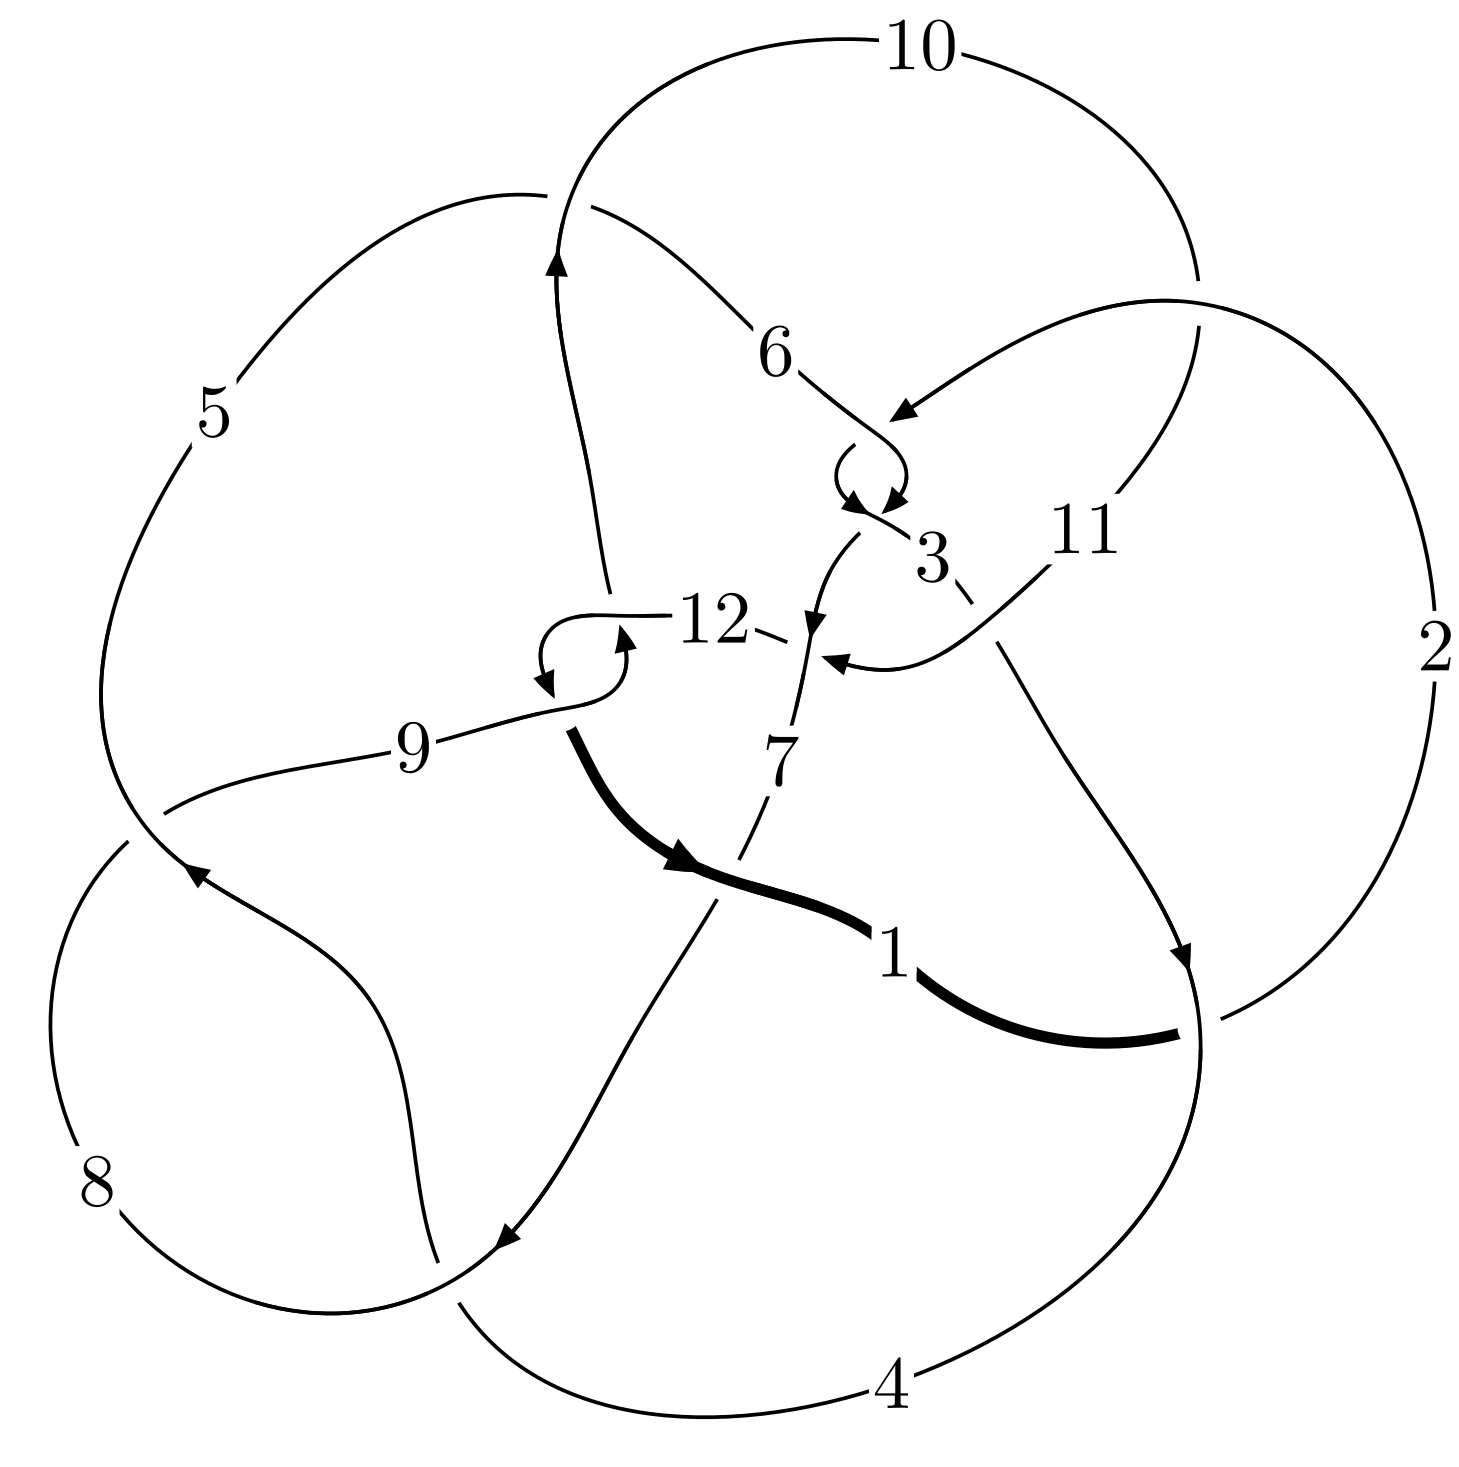
\includegraphics[width=112pt]{../../../GIT/diagram.site/Diagrams/png/1781_12a_0980.png}\\
\ \ \ A knot diagram\footnotemark}&
\allowdisplaybreaks
\textbf{Linearized knot diagam} \\
\cline{2-2}
 &
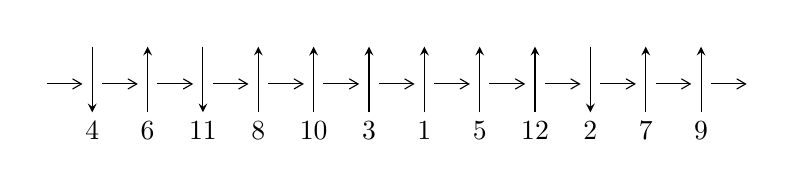
\begin{tikzpicture}[x=20pt, y=17pt]
	% nodes
	\node (C0) at (0, 0) {};
	\node (C1) at (1, 0) {};
	\node (C1U) at (1, +1) {};
	\node (C1D) at (1, -1) {4};

	\node (C2) at (2, 0) {};
	\node (C2U) at (2, +1) {};
	\node (C2D) at (2, -1) {6};

	\node (C3) at (3, 0) {};
	\node (C3U) at (3, +1) {};
	\node (C3D) at (3, -1) {11};

	\node (C4) at (4, 0) {};
	\node (C4U) at (4, +1) {};
	\node (C4D) at (4, -1) {8};

	\node (C5) at (5, 0) {};
	\node (C5U) at (5, +1) {};
	\node (C5D) at (5, -1) {10};

	\node (C6) at (6, 0) {};
	\node (C6U) at (6, +1) {};
	\node (C6D) at (6, -1) {3};

	\node (C7) at (7, 0) {};
	\node (C7U) at (7, +1) {};
	\node (C7D) at (7, -1) {1};

	\node (C8) at (8, 0) {};
	\node (C8U) at (8, +1) {};
	\node (C8D) at (8, -1) {5};

	\node (C9) at (9, 0) {};
	\node (C9U) at (9, +1) {};
	\node (C9D) at (9, -1) {12};

	\node (C10) at (10, 0) {};
	\node (C10U) at (10, +1) {};
	\node (C10D) at (10, -1) {2};

	\node (C11) at (11, 0) {};
	\node (C11U) at (11, +1) {};
	\node (C11D) at (11, -1) {7};

	\node (C12) at (12, 0) {};
	\node (C12U) at (12, +1) {};
	\node (C12D) at (12, -1) {9};
	\node (C13) at (13, 0) {};

	% arrows
	\draw[->,>={angle 60}]
	(C0) edge (C1) (C1) edge (C2) (C2) edge (C3) (C3) edge (C4) (C4) edge (C5) (C5) edge (C6) (C6) edge (C7) (C7) edge (C8) (C8) edge (C9) (C9) edge (C10) (C10) edge (C11) (C11) edge (C12) (C12) edge (C13) ;	\draw[->,>=stealth]
	(C1U) edge (C1D) (C2D) edge (C2U) (C3U) edge (C3D) (C4D) edge (C4U) (C5D) edge (C5U) (C6D) edge (C6U) (C7D) edge (C7U) (C8D) edge (C8U) (C9D) edge (C9U) (C10U) edge (C10D) (C11D) edge (C11U) (C12D) edge (C12U) ;
	\end{tikzpicture} \\
\hhline{~~} \\& 
\textbf{Solving Sequence} \\ \cline{2-2} 
 &
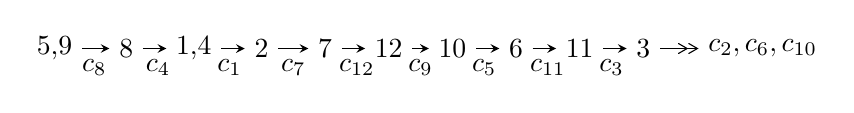
\begin{tikzpicture}[x=23pt, y=7pt]
	% node
	\node (A0) at (-1/8, 0) {5,9};
	\node (A1) at (1, 0) {8};
	\node (A2) at (33/16, 0) {1,4};
	\node (A3) at (25/8, 0) {2};
	\node (A4) at (33/8, 0) {7};
	\node (A5) at (41/8, 0) {12};
	\node (A6) at (49/8, 0) {10};
	\node (A7) at (57/8, 0) {6};
	\node (A8) at (65/8, 0) {11};
	\node (A9) at (73/8, 0) {3};
	\node (C1) at (1/2, -1) {$c_{8}$};
	\node (C2) at (3/2, -1) {$c_{4}$};
	\node (C3) at (21/8, -1) {$c_{1}$};
	\node (C4) at (29/8, -1) {$c_{7}$};
	\node (C5) at (37/8, -1) {$c_{12}$};
	\node (C6) at (45/8, -1) {$c_{9}$};
	\node (C7) at (53/8, -1) {$c_{5}$};
	\node (C8) at (61/8, -1) {$c_{11}$};
	\node (C9) at (69/8, -1) {$c_{3}$};
	\node (A10) at (11, 0) {$c_{2},c_{6},c_{10}$};

	% edge
	\draw[->,>=stealth]	
	(A0) edge (A1) (A1) edge (A2) (A2) edge (A3) (A3) edge (A4) (A4) edge (A5) (A5) edge (A6) (A6) edge (A7) (A7) edge (A8) (A8) edge (A9) ;
	\draw[->>,>={angle 60}]	
	(A9) edge (A10);
\end{tikzpicture} \\ 

\end{tabular} \\

\footnotetext{
The image of knot diagram is generated by the software ``\textbf{Draw programme}" developed by Andrew Bartholomew(\url{http://www.layer8.co.uk/maths/draw/index.htm\#Running-draw}), where we modified some parts for our purpose(\url{https://github.com/CATsTAILs/LinksPainter}).
}\phantom \\ \newline 
\centering \textbf{Ideals for irreducible components\footnotemark of $X_{\text{par}}$} 
 
\begin{align*}
I^u_{1}&=\langle 
-6.36657\times10^{1094} u^{178}-6.23884\times10^{1094} u^{177}+\cdots+5.80635\times10^{1093} b+2.12651\times10^{1098},\\
\phantom{I^u_{1}}&\phantom{= \langle  }-9.79404\times10^{1098} u^{178}-2.54297\times10^{1099} u^{177}+\cdots+1.03893\times10^{1098} a+4.07247\times10^{1103},\\
\phantom{I^u_{1}}&\phantom{= \langle  }u^{179}+u^{178}+\cdots-56442 u+17893\rangle \\
I^u_{2}&=\langle 
-3.77559\times10^{62} u^{50}+1.00246\times10^{63} u^{49}+\cdots+1.99308\times10^{62} b+1.21732\times10^{63},\\
\phantom{I^u_{2}}&\phantom{= \langle  }-1.54082\times10^{61} u^{50}+1.52437\times10^{62} u^{49}+\cdots+2.84726\times10^{61} a+2.21864\times10^{62},\\
\phantom{I^u_{2}}&\phantom{= \langle  }u^{51}-14 u^{49}+\cdots+4 u-1\rangle \\
\\
\end{align*}
\raggedright * 2 irreducible components of $\dim_{\mathbb{C}}=0$, with total 230 representations.\\
\footnotetext{All coefficients of polynomials are rational numbers. But the coefficients are sometimes approximated in decimal forms when there is not enough margin.}
\newpage
\renewcommand{\arraystretch}{1}
\centering \section*{I. $I^u_{1}= \langle -6.37\times10^{1094} u^{178}-6.24\times10^{1094} u^{177}+\cdots+5.81\times10^{1093} b+2.13\times10^{1098},\;-9.79\times10^{1098} u^{178}-2.54\times10^{1099} u^{177}+\cdots+1.04\times10^{1098} a+4.07\times10^{1103},\;u^{179}+u^{178}+\cdots-56442 u+17893 \rangle$}
\flushleft \textbf{(i) Arc colorings}\\
\begin{tabular}{m{7pt} m{180pt} m{7pt} m{180pt} }
\flushright $a_{5}=$&$\begin{pmatrix}0\\u\end{pmatrix}$ \\
\flushright $a_{9}=$&$\begin{pmatrix}1\\0\end{pmatrix}$ \\
\flushright $a_{8}=$&$\begin{pmatrix}1\\u^2\end{pmatrix}$ \\
\flushright $a_{1}=$&$\begin{pmatrix}9.42704 u^{178}+24.4768 u^{177}+\cdots+942651. u-391987.\\10.9648 u^{178}+10.7449 u^{177}+\cdots-167474. u-36623.9\end{pmatrix}$ \\
\flushright $a_{4}=$&$\begin{pmatrix}- u\\- u^3+u\end{pmatrix}$ \\
\flushright $a_{2}=$&$\begin{pmatrix}-0.915545 u^{178}+12.3950 u^{177}+\cdots+965308. u-313140.\\14.0361 u^{178}+15.3675 u^{177}+\cdots-103237. u-84350.7\end{pmatrix}$ \\
\flushright $a_{7}=$&$\begin{pmatrix}-5.94953 u^{178}+9.95972 u^{177}+\cdots+1.28611\times10^{6} u-383601.\\4.14236 u^{178}+4.34252 u^{177}+\cdots-74669.5 u-15655.1\end{pmatrix}$ \\
\flushright $a_{12}=$&$\begin{pmatrix}-1.53779 u^{178}+13.7319 u^{177}+\cdots+1.11013\times10^{6} u-355363.\\10.9648 u^{178}+10.7449 u^{177}+\cdots-167474. u-36623.9\end{pmatrix}$ \\
\flushright $a_{10}=$&$\begin{pmatrix}14.7973 u^{178}+21.7781 u^{177}+\cdots+246198. u-211700.\\16.1247 u^{178}+25.8989 u^{177}+\cdots+467075. u-284144.\end{pmatrix}$ \\
\flushright $a_{6}=$&$\begin{pmatrix}11.6170 u^{178}+8.59561 u^{177}+\cdots-351438. u+7966.34\\-5.98509 u^{178}-12.6327 u^{177}+\cdots-337985. u+167001.\end{pmatrix}$ \\
\flushright $a_{11}=$&$\begin{pmatrix}13.7445 u^{178}+17.0895 u^{177}+\cdots-7907.38 u-109987.\\4.88861 u^{178}+9.90097 u^{177}+\cdots+304402. u-136238.\end{pmatrix}$ \\
\flushright $a_{3}=$&$\begin{pmatrix}-14.0038 u^{178}-19.3801 u^{177}+\cdots-264116. u+217958.\\-12.5597 u^{178}-23.7283 u^{177}+\cdots-635008. u+309138.\end{pmatrix}$\\&\end{tabular}
\flushleft \textbf{(ii) Obstruction class $= -1$}\\~\\
\flushleft \textbf{(iii) Cusp Shapes $= -66.0926 u^{178}-118.720 u^{177}+\cdots-2.78433\times10^{6} u+1.47029\times10^{6}$}\\~\\
\newpage\renewcommand{\arraystretch}{1}
\flushleft \textbf{(iv) u-Polynomials at the component}\newline \\
\begin{tabular}{m{50pt}|m{274pt}}
Crossings & \hspace{64pt}u-Polynomials at each crossing \\
\hline $$\begin{aligned}c_{1}\end{aligned}$$&$\begin{aligned}
&u^{179}-13 u^{178}+\cdots+89605118959 u-3985097653
\end{aligned}$\\
\hline $$\begin{aligned}c_{2},c_{6}\end{aligned}$$&$\begin{aligned}
&u^{179}-2 u^{178}+\cdots-29 u+1
\end{aligned}$\\
\hline $$\begin{aligned}c_{3}\end{aligned}$$&$\begin{aligned}
&u^{179}-3 u^{178}+\cdots-36410582 u-8875751
\end{aligned}$\\
\hline $$\begin{aligned}c_{4},c_{8}\end{aligned}$$&$\begin{aligned}
&u^{179}- u^{178}+\cdots-56442 u-17893
\end{aligned}$\\
\hline $$\begin{aligned}c_{5}\end{aligned}$$&$\begin{aligned}
&u^{179}+2 u^{178}+\cdots-2211089289451 u+384248970739
\end{aligned}$\\
\hline $$\begin{aligned}c_{7}\end{aligned}$$&$\begin{aligned}
&u^{179}-15 u^{177}+\cdots-5920100 u-554293
\end{aligned}$\\
\hline $$\begin{aligned}c_{9},c_{12}\end{aligned}$$&$\begin{aligned}
&u^{179}-8 u^{178}+\cdots+129296 u-16120
\end{aligned}$\\
\hline $$\begin{aligned}c_{10}\end{aligned}$$&$\begin{aligned}
&u^{179}+9 u^{178}+\cdots+72454819 u-599297
\end{aligned}$\\
\hline $$\begin{aligned}c_{11}\end{aligned}$$&$\begin{aligned}
&u^{179}-32 u^{177}+\cdots+11845686300 u+9627412451
\end{aligned}$\\
\hline
\end{tabular}\\~\\
\newpage\renewcommand{\arraystretch}{1}
\flushleft \textbf{(v) Riley Polynomials at the component}\newline \\
\begin{tabular}{m{50pt}|m{274pt}}
Crossings & \hspace{64pt}Riley Polynomials at each crossing \\
\hline $$\begin{aligned}c_{1}\end{aligned}$$&$\begin{aligned}
&y^{179}+85 y^{178}+\cdots+1.82\times10^{21} y-1.59\times10^{19}
\end{aligned}$\\
\hline $$\begin{aligned}c_{2},c_{6}\end{aligned}$$&$\begin{aligned}
&y^{179}-120 y^{178}+\cdots-119 y-1
\end{aligned}$\\
\hline $$\begin{aligned}c_{3}\end{aligned}$$&$\begin{aligned}
&y^{179}+55 y^{178}+\cdots-2321290894230492 y-78778955814001
\end{aligned}$\\
\hline $$\begin{aligned}c_{4},c_{8}\end{aligned}$$&$\begin{aligned}
&y^{179}-111 y^{178}+\cdots+20997393572 y-320159449
\end{aligned}$\\
\hline $$\begin{aligned}c_{5}\end{aligned}$$&$\begin{aligned}
&y^{179}-88 y^{178}+\cdots+7.44\times10^{24} y-1.48\times10^{23}
\end{aligned}$\\
\hline $$\begin{aligned}c_{7}\end{aligned}$$&$\begin{aligned}
&y^{179}-30 y^{178}+\cdots+17033627997446 y-307240729849
\end{aligned}$\\
\hline $$\begin{aligned}c_{9},c_{12}\end{aligned}$$&$\begin{aligned}
&y^{179}+108 y^{178}+\cdots+1685942496 y-259854400
\end{aligned}$\\
\hline $$\begin{aligned}c_{10}\end{aligned}$$&$\begin{aligned}
&y^{179}+71 y^{178}+\cdots+1040989262644787 y-359156894209
\end{aligned}$\\
\hline $$\begin{aligned}c_{11}\end{aligned}$$&$\begin{aligned}
&y^{179}-64 y^{178}+\cdots+2.73\times10^{21} y-9.27\times10^{19}
\end{aligned}$\\
\hline
\end{tabular}\\~\\
\newpage\flushleft \textbf{(vi) Complex Volumes and Cusp Shapes}
$$\begin{array}{c|c|c}  
\text{Solutions to }I^u_{1}& \I (\text{vol} + \sqrt{-1}CS) & \text{Cusp shape}\\
 \hline 
\begin{aligned}
u &= \phantom{-}0.191510 + 0.975345 I \\
a &= \phantom{-}0.118476 - 0.197233 I \\
b &= -0.947699 + 0.317526 I\end{aligned}
 & \phantom{-}4.79126 - 1.30542 I & \phantom{-0.000000 } 0 \\ \hline\begin{aligned}
u &= \phantom{-}0.191510 - 0.975345 I \\
a &= \phantom{-}0.118476 + 0.197233 I \\
b &= -0.947699 - 0.317526 I\end{aligned}
 & \phantom{-}4.79126 + 1.30542 I & \phantom{-0.000000 } 0 \\ \hline\begin{aligned}
u &= \phantom{-}0.375219 + 0.907827 I \\
a &= \phantom{-}0.100769 + 0.225810 I \\
b &= \phantom{-}0.188848 - 1.139220 I\end{aligned}
 & -5.45462 - 0.67402 I & \phantom{-0.000000 } 0 \\ \hline\begin{aligned}
u &= \phantom{-}0.375219 - 0.907827 I \\
a &= \phantom{-}0.100769 - 0.225810 I \\
b &= \phantom{-}0.188848 + 1.139220 I\end{aligned}
 & -5.45462 + 0.67402 I & \phantom{-0.000000 } 0 \\ \hline\begin{aligned}
u &= -0.946996 + 0.254827 I \\
a &= \phantom{-}1.339280 - 0.439621 I \\
b &= \phantom{-}0.062365 - 0.796418 I\end{aligned}
 & \phantom{-}0.388929 - 0.512029 I & \phantom{-0.000000 } 0 \\ \hline\begin{aligned}
u &= -0.946996 - 0.254827 I \\
a &= \phantom{-}1.339280 + 0.439621 I \\
b &= \phantom{-}0.062365 + 0.796418 I\end{aligned}
 & \phantom{-}0.388929 + 0.512029 I & \phantom{-0.000000 } 0 \\ \hline\begin{aligned}
u &= -0.975305 + 0.098384 I \\
a &= -0.38360 + 1.53179 I \\
b &= -0.06444 + 2.27255 I\end{aligned}
 & \phantom{-}3.17314 - 5.97245 I & \phantom{-0.000000 } 0 \\ \hline\begin{aligned}
u &= -0.975305 - 0.098384 I \\
a &= -0.38360 - 1.53179 I \\
b &= -0.06444 - 2.27255 I\end{aligned}
 & \phantom{-}3.17314 + 5.97245 I & \phantom{-0.000000 } 0 \\ \hline\begin{aligned}
u &= \phantom{-}0.694979 + 0.746273 I \\
a &= \phantom{-}0.297989 - 0.458844 I \\
b &= \phantom{-}0.586488 - 1.068690 I\end{aligned}
 & -2.89144 - 0.09708 I & \phantom{-0.000000 } 0 \\ \hline\begin{aligned}
u &= \phantom{-}0.694979 - 0.746273 I \\
a &= \phantom{-}0.297989 + 0.458844 I \\
b &= \phantom{-}0.586488 + 1.068690 I\end{aligned}
 & -2.89144 + 0.09708 I & \phantom{-0.000000 } 0\\
 \hline 
 \end{array}$$\newpage$$\begin{array}{c|c|c}  
\text{Solutions to }I^u_{1}& \I (\text{vol} + \sqrt{-1}CS) & \text{Cusp shape}\\
 \hline 
\begin{aligned}
u &= -0.116062 + 1.015720 I \\
a &= -0.206539 - 0.424655 I \\
b &= -0.341854 + 1.180290 I\end{aligned}
 & -1.80573 - 3.51908 I & \phantom{-0.000000 } 0 \\ \hline\begin{aligned}
u &= -0.116062 - 1.015720 I \\
a &= -0.206539 + 0.424655 I \\
b &= -0.341854 - 1.180290 I\end{aligned}
 & -1.80573 + 3.51908 I & \phantom{-0.000000 } 0 \\ \hline\begin{aligned}
u &= -1.022450 + 0.148399 I \\
a &= -1.06383 + 1.34144 I \\
b &= -0.430224 + 0.883668 I\end{aligned}
 & -0.201149 - 1.026760 I & \phantom{-0.000000 } 0 \\ \hline\begin{aligned}
u &= -1.022450 - 0.148399 I \\
a &= -1.06383 - 1.34144 I \\
b &= -0.430224 - 0.883668 I\end{aligned}
 & -0.201149 + 1.026760 I & \phantom{-0.000000 } 0 \\ \hline\begin{aligned}
u &= \phantom{-}1.04026\phantom{ +0.000000I} \\
a &= -1.37597\phantom{ +0.000000I} \\
b &= -1.38131\phantom{ +0.000000I}\end{aligned}
 & \phantom{-}6.45100\phantom{ +0.000000I} & \phantom{-0.000000 } 0 \\ \hline\begin{aligned}
u &= \phantom{-}1.028270 + 0.191790 I \\
a &= -1.69759 - 1.10708 I \\
b &= -0.500660 - 1.253070 I\end{aligned}
 & \phantom{-}1.08260 + 5.29643 I & \phantom{-0.000000 } 0 \\ \hline\begin{aligned}
u &= \phantom{-}1.028270 - 0.191790 I \\
a &= -1.69759 + 1.10708 I \\
b &= -0.500660 + 1.253070 I\end{aligned}
 & \phantom{-}1.08260 - 5.29643 I & \phantom{-0.000000 } 0 \\ \hline\begin{aligned}
u &= -0.395308 + 0.868172 I \\
a &= -0.043328 - 0.380665 I \\
b &= \phantom{-}0.007344 + 1.268340 I\end{aligned}
 & -3.54685 - 4.04229 I & \phantom{-0.000000 } 0 \\ \hline\begin{aligned}
u &= -0.395308 - 0.868172 I \\
a &= -0.043328 + 0.380665 I \\
b &= \phantom{-}0.007344 - 1.268340 I\end{aligned}
 & -3.54685 + 4.04229 I & \phantom{-0.000000 } 0 \\ \hline\begin{aligned}
u &= \phantom{-}0.234582 + 0.914258 I \\
a &= \phantom{-}0.533039 + 0.548870 I \\
b &= -0.331503 - 1.024530 I\end{aligned}
 & \phantom{-}0.38897 + 1.81521 I & \phantom{-0.000000 } 0\\
 \hline 
 \end{array}$$\newpage$$\begin{array}{c|c|c}  
\text{Solutions to }I^u_{1}& \I (\text{vol} + \sqrt{-1}CS) & \text{Cusp shape}\\
 \hline 
\begin{aligned}
u &= \phantom{-}0.234582 - 0.914258 I \\
a &= \phantom{-}0.533039 - 0.548870 I \\
b &= -0.331503 + 1.024530 I\end{aligned}
 & \phantom{-}0.38897 - 1.81521 I & \phantom{-0.000000 } 0 \\ \hline\begin{aligned}
u &= \phantom{-}1.055370 + 0.060677 I \\
a &= -1.94809 + 0.29399 I \\
b &= -0.845985 + 0.870023 I\end{aligned}
 & \phantom{-}6.97891 - 0.56802 I & \phantom{-0.000000 } 0 \\ \hline\begin{aligned}
u &= \phantom{-}1.055370 - 0.060677 I \\
a &= -1.94809 - 0.29399 I \\
b &= -0.845985 - 0.870023 I\end{aligned}
 & \phantom{-}6.97891 + 0.56802 I & \phantom{-0.000000 } 0 \\ \hline\begin{aligned}
u &= -1.044820 + 0.204391 I \\
a &= -1.96034 + 0.56484 I \\
b &= -0.86099 + 1.44495 I\end{aligned}
 & \phantom{-}4.45508 - 5.23948 I & \phantom{-0.000000 } 0 \\ \hline\begin{aligned}
u &= -1.044820 - 0.204391 I \\
a &= -1.96034 - 0.56484 I \\
b &= -0.86099 - 1.44495 I\end{aligned}
 & \phantom{-}4.45508 + 5.23948 I & \phantom{-0.000000 } 0 \\ \hline\begin{aligned}
u &= \phantom{-}0.788571 + 0.493295 I \\
a &= \phantom{-}1.284810 + 0.477379 I \\
b &= -0.308034 + 0.691588 I\end{aligned}
 & \phantom{-}1.48051 - 1.02975 I & \phantom{-0.000000 } 0 \\ \hline\begin{aligned}
u &= \phantom{-}0.788571 - 0.493295 I \\
a &= \phantom{-}1.284810 - 0.477379 I \\
b &= -0.308034 - 0.691588 I\end{aligned}
 & \phantom{-}1.48051 + 1.02975 I & \phantom{-0.000000 } 0 \\ \hline\begin{aligned}
u &= -0.925596 + 0.013084 I \\
a &= -0.698849 + 0.532216 I \\
b &= -0.249552 - 1.386880 I\end{aligned}
 & -0.903421 + 0.405747 I & \phantom{-0.000000 } 0 \\ \hline\begin{aligned}
u &= -0.925596 - 0.013084 I \\
a &= -0.698849 - 0.532216 I \\
b &= -0.249552 + 1.386880 I\end{aligned}
 & -0.903421 - 0.405747 I & \phantom{-0.000000 } 0 \\ \hline\begin{aligned}
u &= -0.484278 + 0.787433 I \\
a &= -0.066392 + 0.304210 I \\
b &= \phantom{-}0.580563 + 1.201390 I\end{aligned}
 & \phantom{-}1.31125 + 7.29801 I & \phantom{-0.000000 } 0\\
 \hline 
 \end{array}$$\newpage$$\begin{array}{c|c|c}  
\text{Solutions to }I^u_{1}& \I (\text{vol} + \sqrt{-1}CS) & \text{Cusp shape}\\
 \hline 
\begin{aligned}
u &= -0.484278 - 0.787433 I \\
a &= -0.066392 - 0.304210 I \\
b &= \phantom{-}0.580563 - 1.201390 I\end{aligned}
 & \phantom{-}1.31125 - 7.29801 I & \phantom{-0.000000 } 0 \\ \hline\begin{aligned}
u &= \phantom{-}1.072350 + 0.115906 I \\
a &= \phantom{-}1.86158 - 1.10211 I \\
b &= \phantom{-}0.369327 + 1.113980 I\end{aligned}
 & \phantom{-}6.99350 + 9.59579 I & \phantom{-0.000000 } 0 \\ \hline\begin{aligned}
u &= \phantom{-}1.072350 - 0.115906 I \\
a &= \phantom{-}1.86158 + 1.10211 I \\
b &= \phantom{-}0.369327 - 1.113980 I\end{aligned}
 & \phantom{-}6.99350 - 9.59579 I & \phantom{-0.000000 } 0 \\ \hline\begin{aligned}
u &= -0.797805 + 0.734362 I \\
a &= -0.697193 - 1.051610 I \\
b &= -0.187724 + 0.468601 I\end{aligned}
 & \phantom{-}2.22385 - 4.22991 I & \phantom{-0.000000 } 0 \\ \hline\begin{aligned}
u &= -0.797805 - 0.734362 I \\
a &= -0.697193 + 1.051610 I \\
b &= -0.187724 - 0.468601 I\end{aligned}
 & \phantom{-}2.22385 + 4.22991 I & \phantom{-0.000000 } 0 \\ \hline\begin{aligned}
u &= -1.089330 + 0.082965 I \\
a &= \phantom{-}2.11407 + 0.72636 I \\
b &= \phantom{-}0.321990 - 0.997454 I\end{aligned}
 & \phantom{-}3.15679 - 3.44042 I & \phantom{-0.000000 } 0 \\ \hline\begin{aligned}
u &= -1.089330 - 0.082965 I \\
a &= \phantom{-}2.11407 - 0.72636 I \\
b &= \phantom{-}0.321990 + 0.997454 I\end{aligned}
 & \phantom{-}3.15679 + 3.44042 I & \phantom{-0.000000 } 0 \\ \hline\begin{aligned}
u &= \phantom{-}1.068920 + 0.230795 I \\
a &= -1.58462 - 0.59878 I \\
b &= -0.76662 - 1.31287 I\end{aligned}
 & \phantom{-}1.43841 + 4.21089 I & \phantom{-0.000000 } 0 \\ \hline\begin{aligned}
u &= \phantom{-}1.068920 - 0.230795 I \\
a &= -1.58462 + 0.59878 I \\
b &= -0.76662 + 1.31287 I\end{aligned}
 & \phantom{-}1.43841 - 4.21089 I & \phantom{-0.000000 } 0 \\ \hline\begin{aligned}
u &= \phantom{-}0.893618 + 0.137441 I \\
a &= \phantom{-}0.123624 - 0.813825 I \\
b &= \phantom{-}0.11336 - 1.63515 I\end{aligned}
 & -0.83450 + 3.38680 I & \phantom{-0.000000 } 0\\
 \hline 
 \end{array}$$\newpage$$\begin{array}{c|c|c}  
\text{Solutions to }I^u_{1}& \I (\text{vol} + \sqrt{-1}CS) & \text{Cusp shape}\\
 \hline 
\begin{aligned}
u &= \phantom{-}0.893618 - 0.137441 I \\
a &= \phantom{-}0.123624 + 0.813825 I \\
b &= \phantom{-}0.11336 + 1.63515 I\end{aligned}
 & -0.83450 - 3.38680 I & \phantom{-0.000000 } 0 \\ \hline\begin{aligned}
u &= \phantom{-}0.009597 + 0.902263 I \\
a &= \phantom{-}0.631888 - 0.476415 I \\
b &= -0.180297 + 1.161690 I\end{aligned}
 & -1.17829 - 1.51049 I & \phantom{-0.000000 } 0 \\ \hline\begin{aligned}
u &= \phantom{-}0.009597 - 0.902263 I \\
a &= \phantom{-}0.631888 + 0.476415 I \\
b &= -0.180297 - 1.161690 I\end{aligned}
 & -1.17829 + 1.51049 I & \phantom{-0.000000 } 0 \\ \hline\begin{aligned}
u &= -0.795290 + 0.404762 I \\
a &= -1.51504 - 0.62301 I \\
b &= -0.470451 + 1.030880 I\end{aligned}
 & -0.79294 - 2.75953 I & \phantom{-0.000000 } 0 \\ \hline\begin{aligned}
u &= -0.795290 - 0.404762 I \\
a &= -1.51504 + 0.62301 I \\
b &= -0.470451 - 1.030880 I\end{aligned}
 & -0.79294 + 2.75953 I & \phantom{-0.000000 } 0 \\ \hline\begin{aligned}
u &= -0.885818 + 0.081819 I \\
a &= -2.65694 - 0.88690 I \\
b &= -0.199628 - 0.659956 I\end{aligned}
 & \phantom{-}1.99440 - 3.25458 I & \phantom{-0.000000 } 0 \\ \hline\begin{aligned}
u &= -0.885818 - 0.081819 I \\
a &= -2.65694 + 0.88690 I \\
b &= -0.199628 + 0.659956 I\end{aligned}
 & \phantom{-}1.99440 + 3.25458 I & \phantom{-0.000000 } 0 \\ \hline\begin{aligned}
u &= -0.790038 + 0.400109 I \\
a &= \phantom{-}2.06005 + 0.39546 I \\
b &= \phantom{-}1.143800 - 0.529162 I\end{aligned}
 & \phantom{-}4.11819 + 1.31718 I & \phantom{-0.000000 } 0 \\ \hline\begin{aligned}
u &= -0.790038 - 0.400109 I \\
a &= \phantom{-}2.06005 - 0.39546 I \\
b &= \phantom{-}1.143800 + 0.529162 I\end{aligned}
 & \phantom{-}4.11819 - 1.31718 I & \phantom{-0.000000 } 0 \\ \hline\begin{aligned}
u &= \phantom{-}0.368314 + 0.786480 I \\
a &= -0.055277 - 1.054380 I \\
b &= -0.30421 + 1.38213 I\end{aligned}
 & -0.75429 - 5.59436 I & \phantom{-0.000000 } 0\\
 \hline 
 \end{array}$$\newpage$$\begin{array}{c|c|c}  
\text{Solutions to }I^u_{1}& \I (\text{vol} + \sqrt{-1}CS) & \text{Cusp shape}\\
 \hline 
\begin{aligned}
u &= \phantom{-}0.368314 - 0.786480 I \\
a &= -0.055277 + 1.054380 I \\
b &= -0.30421 - 1.38213 I\end{aligned}
 & -0.75429 + 5.59436 I & \phantom{-0.000000 } 0 \\ \hline\begin{aligned}
u &= \phantom{-}1.141300 + 0.083051 I \\
a &= \phantom{-}1.57053 - 0.51047 I \\
b &= \phantom{-}0.442379 + 0.865177 I\end{aligned}
 & \phantom{-}8.26946 - 1.83716 I & \phantom{-0.000000 } 0 \\ \hline\begin{aligned}
u &= \phantom{-}1.141300 - 0.083051 I \\
a &= \phantom{-}1.57053 + 0.51047 I \\
b &= \phantom{-}0.442379 - 0.865177 I\end{aligned}
 & \phantom{-}8.26946 + 1.83716 I & \phantom{-0.000000 } 0 \\ \hline\begin{aligned}
u &= -0.276710 + 1.112220 I \\
a &= \phantom{-}0.103126 + 0.516037 I \\
b &= -0.626442 - 1.133640 I\end{aligned}
 & \phantom{-}2.36728 + 4.36232 I & \phantom{-0.000000 } 0 \\ \hline\begin{aligned}
u &= -0.276710 - 1.112220 I \\
a &= \phantom{-}0.103126 - 0.516037 I \\
b &= -0.626442 + 1.133640 I\end{aligned}
 & \phantom{-}2.36728 - 4.36232 I & \phantom{-0.000000 } 0 \\ \hline\begin{aligned}
u &= \phantom{-}0.275018 + 0.801148 I \\
a &= -0.073003 + 0.909575 I \\
b &= \phantom{-}0.729499 - 0.190679 I\end{aligned}
 & \phantom{-}6.49608 + 9.46240 I & \phantom{-0.000000 } 0 \\ \hline\begin{aligned}
u &= \phantom{-}0.275018 - 0.801148 I \\
a &= -0.073003 - 0.909575 I \\
b &= \phantom{-}0.729499 + 0.190679 I\end{aligned}
 & \phantom{-}6.49608 - 9.46240 I & \phantom{-0.000000 } 0 \\ \hline\begin{aligned}
u &= \phantom{-}0.951414 + 0.657939 I \\
a &= \phantom{-}1.68782 - 0.15946 I \\
b &= \phantom{-}0.796773 + 0.916864 I\end{aligned}
 & -2.13218 + 5.45756 I & \phantom{-0.000000 } 0 \\ \hline\begin{aligned}
u &= \phantom{-}0.951414 - 0.657939 I \\
a &= \phantom{-}1.68782 + 0.15946 I \\
b &= \phantom{-}0.796773 - 0.916864 I\end{aligned}
 & -2.13218 - 5.45756 I & \phantom{-0.000000 } 0 \\ \hline\begin{aligned}
u &= -0.144554 + 1.149850 I \\
a &= \phantom{-}0.216287 - 0.174095 I \\
b &= \phantom{-}0.510759 + 0.957280 I\end{aligned}
 & \phantom{-}4.18934 + 2.17036 I & \phantom{-0.000000 } 0\\
 \hline 
 \end{array}$$\newpage$$\begin{array}{c|c|c}  
\text{Solutions to }I^u_{1}& \I (\text{vol} + \sqrt{-1}CS) & \text{Cusp shape}\\
 \hline 
\begin{aligned}
u &= -0.144554 - 1.149850 I \\
a &= \phantom{-}0.216287 + 0.174095 I \\
b &= \phantom{-}0.510759 - 0.957280 I\end{aligned}
 & \phantom{-}4.18934 - 2.17036 I & \phantom{-0.000000 } 0 \\ \hline\begin{aligned}
u &= -1.037100 + 0.529592 I \\
a &= \phantom{-}1.82446 - 0.08271 I \\
b &= \phantom{-}0.89977 - 1.20050 I\end{aligned}
 & \phantom{-}3.01705 - 12.23120 I & \phantom{-0.000000 } 0 \\ \hline\begin{aligned}
u &= -1.037100 - 0.529592 I \\
a &= \phantom{-}1.82446 + 0.08271 I \\
b &= \phantom{-}0.89977 + 1.20050 I\end{aligned}
 & \phantom{-}3.01705 + 12.23120 I & \phantom{-0.000000 } 0 \\ \hline\begin{aligned}
u &= \phantom{-}0.346376 + 0.750958 I \\
a &= -0.198505 + 0.241752 I \\
b &= -0.413113 - 1.216860 I\end{aligned}
 & \phantom{-}0.41963 + 5.33170 I & \phantom{-0.000000 } 0 \\ \hline\begin{aligned}
u &= \phantom{-}0.346376 - 0.750958 I \\
a &= -0.198505 - 0.241752 I \\
b &= -0.413113 + 1.216860 I\end{aligned}
 & \phantom{-}0.41963 - 5.33170 I & \phantom{-0.000000 } 0 \\ \hline\begin{aligned}
u &= -0.816915 + 0.127889 I \\
a &= \phantom{-}1.23300 - 1.70481 I \\
b &= \phantom{-}0.47885 - 1.67712 I\end{aligned}
 & \phantom{-}2.85122 + 4.76181 I & \phantom{-0.000000 } 0 \\ \hline\begin{aligned}
u &= -0.816915 - 0.127889 I \\
a &= \phantom{-}1.23300 + 1.70481 I \\
b &= \phantom{-}0.47885 + 1.67712 I\end{aligned}
 & \phantom{-}2.85122 - 4.76181 I & \phantom{-0.000000 } 0 \\ \hline\begin{aligned}
u &= \phantom{-}0.822937 + 0.015885 I \\
a &= \phantom{-}0.360949 - 0.120252 I \\
b &= -0.17133 + 1.46839 I\end{aligned}
 & -0.05020 - 4.15344 I & \phantom{-0.000000 } 0 \\ \hline\begin{aligned}
u &= \phantom{-}0.822937 - 0.015885 I \\
a &= \phantom{-}0.360949 + 0.120252 I \\
b &= -0.17133 - 1.46839 I\end{aligned}
 & -0.05020 + 4.15344 I & \phantom{-0.000000 } 0 \\ \hline\begin{aligned}
u &= \phantom{-}1.078340 + 0.479447 I \\
a &= -1.123520 - 0.089759 I \\
b &= -0.52947 - 1.37164 I\end{aligned}
 & \phantom{-}1.63166 + 6.37273 I & \phantom{-0.000000 } 0\\
 \hline 
 \end{array}$$\newpage$$\begin{array}{c|c|c}  
\text{Solutions to }I^u_{1}& \I (\text{vol} + \sqrt{-1}CS) & \text{Cusp shape}\\
 \hline 
\begin{aligned}
u &= \phantom{-}1.078340 - 0.479447 I \\
a &= -1.123520 + 0.089759 I \\
b &= -0.52947 + 1.37164 I\end{aligned}
 & \phantom{-}1.63166 - 6.37273 I & \phantom{-0.000000 } 0 \\ \hline\begin{aligned}
u &= \phantom{-}0.801770\phantom{ +0.000000I} \\
a &= -2.96835\phantom{ +0.000000I} \\
b &= -1.20745\phantom{ +0.000000I}\end{aligned}
 & \phantom{-}5.37744\phantom{ +0.000000I} & \phantom{-0.000000 } 0 \\ \hline\begin{aligned}
u &= -1.188800 + 0.196438 I \\
a &= -1.25535 + 0.65654 I \\
b &= -0.95789 + 1.37969 I\end{aligned}
 & \phantom{-}5.16568 - 5.08352 I & \phantom{-0.000000 } 0 \\ \hline\begin{aligned}
u &= -1.188800 - 0.196438 I \\
a &= -1.25535 - 0.65654 I \\
b &= -0.95789 - 1.37969 I\end{aligned}
 & \phantom{-}5.16568 + 5.08352 I & \phantom{-0.000000 } 0 \\ \hline\begin{aligned}
u &= \phantom{-}0.772288 + 0.013491 I \\
a &= -2.79080 + 1.53448 I \\
b &= \phantom{-}0.131268 + 0.625517 I\end{aligned}
 & \phantom{-}5.76475 + 8.81745 I & \phantom{-0.000000 } 0 \\ \hline\begin{aligned}
u &= \phantom{-}0.772288 - 0.013491 I \\
a &= -2.79080 - 1.53448 I \\
b &= \phantom{-}0.131268 - 0.625517 I\end{aligned}
 & \phantom{-}5.76475 - 8.81745 I & \phantom{-0.000000 } 0 \\ \hline\begin{aligned}
u &= -1.124030 + 0.494970 I \\
a &= \phantom{-}1.44326 - 0.31578 I \\
b &= \phantom{-}0.280647 - 1.111280 I\end{aligned}
 & -1.17991 - 0.91573 I & \phantom{-0.000000 } 0 \\ \hline\begin{aligned}
u &= -1.124030 - 0.494970 I \\
a &= \phantom{-}1.44326 + 0.31578 I \\
b &= \phantom{-}0.280647 + 1.111280 I\end{aligned}
 & -1.17991 + 0.91573 I & \phantom{-0.000000 } 0 \\ \hline\begin{aligned}
u &= -1.182700 + 0.332842 I \\
a &= -2.19273 + 0.64571 I \\
b &= -0.335844 + 1.057860 I\end{aligned}
 & \phantom{-}0.49381 - 5.85529 I & \phantom{-0.000000 } 0 \\ \hline\begin{aligned}
u &= -1.182700 - 0.332842 I \\
a &= -2.19273 - 0.64571 I \\
b &= -0.335844 - 1.057860 I\end{aligned}
 & \phantom{-}0.49381 + 5.85529 I & \phantom{-0.000000 } 0\\
 \hline 
 \end{array}$$\newpage$$\begin{array}{c|c|c}  
\text{Solutions to }I^u_{1}& \I (\text{vol} + \sqrt{-1}CS) & \text{Cusp shape}\\
 \hline 
\begin{aligned}
u &= -0.706053 + 0.289145 I \\
a &= \phantom{-}0.618666 + 0.412008 I \\
b &= -0.163361 + 0.832838 I\end{aligned}
 & \phantom{-}2.73557 - 3.64954 I & \phantom{-0.000000 } 0 \\ \hline\begin{aligned}
u &= -0.706053 - 0.289145 I \\
a &= \phantom{-}0.618666 - 0.412008 I \\
b &= -0.163361 - 0.832838 I\end{aligned}
 & \phantom{-}2.73557 + 3.64954 I & \phantom{-0.000000 } 0 \\ \hline\begin{aligned}
u &= -0.219861 + 0.728037 I \\
a &= \phantom{-}0.275643 - 1.094810 I \\
b &= \phantom{-}0.538557 + 0.161565 I\end{aligned}
 & \phantom{-}1.77929 - 4.20041 I & \phantom{-0.000000 } 0 \\ \hline\begin{aligned}
u &= -0.219861 - 0.728037 I \\
a &= \phantom{-}0.275643 + 1.094810 I \\
b &= \phantom{-}0.538557 - 0.161565 I\end{aligned}
 & \phantom{-}1.77929 + 4.20041 I & \phantom{-0.000000 } 0 \\ \hline\begin{aligned}
u &= -0.854353 + 0.903285 I \\
a &= \phantom{-}0.399708 - 0.223974 I \\
b &= -0.154240 - 1.091590 I\end{aligned}
 & -0.18011 - 2.39642 I & \phantom{-0.000000 } 0 \\ \hline\begin{aligned}
u &= -0.854353 - 0.903285 I \\
a &= \phantom{-}0.399708 + 0.223974 I \\
b &= -0.154240 + 1.091590 I\end{aligned}
 & -0.18011 + 2.39642 I & \phantom{-0.000000 } 0 \\ \hline\begin{aligned}
u &= \phantom{-}0.126555 + 1.237890 I \\
a &= \phantom{-}0.201374 + 0.261483 I \\
b &= \phantom{-}0.475752 - 1.106210 I\end{aligned}
 & -0.72693 - 8.29143 I & \phantom{-0.000000 } 0 \\ \hline\begin{aligned}
u &= \phantom{-}0.126555 - 1.237890 I \\
a &= \phantom{-}0.201374 - 0.261483 I \\
b &= \phantom{-}0.475752 + 1.106210 I\end{aligned}
 & -0.72693 + 8.29143 I & \phantom{-0.000000 } 0 \\ \hline\begin{aligned}
u &= -0.092167 + 1.243940 I \\
a &= \phantom{-}0.159980 - 0.280420 I \\
b &= \phantom{-}0.534164 + 1.181950 I\end{aligned}
 & \phantom{-}3.6088 + 14.3003 I & \phantom{-0.000000 } 0 \\ \hline\begin{aligned}
u &= -0.092167 - 1.243940 I \\
a &= \phantom{-}0.159980 + 0.280420 I \\
b &= \phantom{-}0.534164 - 1.181950 I\end{aligned}
 & \phantom{-}3.6088 - 14.3003 I & \phantom{-0.000000 } 0\\
 \hline 
 \end{array}$$\newpage$$\begin{array}{c|c|c}  
\text{Solutions to }I^u_{1}& \I (\text{vol} + \sqrt{-1}CS) & \text{Cusp shape}\\
 \hline 
\begin{aligned}
u &= \phantom{-}1.143450 + 0.558703 I \\
a &= \phantom{-}1.50878 + 0.15613 I \\
b &= \phantom{-}0.520565 + 1.074370 I\end{aligned}
 & -3.00244 + 5.99318 I & \phantom{-0.000000 } 0 \\ \hline\begin{aligned}
u &= \phantom{-}1.143450 - 0.558703 I \\
a &= \phantom{-}1.50878 - 0.15613 I \\
b &= \phantom{-}0.520565 - 1.074370 I\end{aligned}
 & -3.00244 - 5.99318 I & \phantom{-0.000000 } 0 \\ \hline\begin{aligned}
u &= \phantom{-}1.182360 + 0.480617 I \\
a &= -1.90987 - 0.05793 I \\
b &= -0.374567 - 1.304610 I\end{aligned}
 & \phantom{-}1.86761 + 10.39370 I & \phantom{-0.000000 } 0 \\ \hline\begin{aligned}
u &= \phantom{-}1.182360 - 0.480617 I \\
a &= -1.90987 + 0.05793 I \\
b &= -0.374567 + 1.304610 I\end{aligned}
 & \phantom{-}1.86761 - 10.39370 I & \phantom{-0.000000 } 0 \\ \hline\begin{aligned}
u &= \phantom{-}1.266980 + 0.271325 I \\
a &= -1.353550 + 0.266542 I \\
b &= -1.170570 + 0.130249 I\end{aligned}
 & \phantom{-}6.26061 + 2.93785 I & \phantom{-0.000000 } 0 \\ \hline\begin{aligned}
u &= \phantom{-}1.266980 - 0.271325 I \\
a &= -1.353550 - 0.266542 I \\
b &= -1.170570 - 0.130249 I\end{aligned}
 & \phantom{-}6.26061 - 2.93785 I & \phantom{-0.000000 } 0 \\ \hline\begin{aligned}
u &= -1.286460 + 0.171895 I \\
a &= -1.59609 - 0.01924 I \\
b &= -1.364240 - 0.155380 I\end{aligned}
 & \phantom{-}9.46041 - 2.58014 I & \phantom{-0.000000 } 0 \\ \hline\begin{aligned}
u &= -1.286460 - 0.171895 I \\
a &= -1.59609 + 0.01924 I \\
b &= -1.364240 + 0.155380 I\end{aligned}
 & \phantom{-}9.46041 + 2.58014 I & \phantom{-0.000000 } 0 \\ \hline\begin{aligned}
u &= -1.249080 + 0.407640 I \\
a &= \phantom{-}1.089510 + 0.531724 I \\
b &= \phantom{-}1.066740 + 0.682532 I\end{aligned}
 & \phantom{-}9.49493 - 1.84699 I & \phantom{-0.000000 } 0 \\ \hline\begin{aligned}
u &= -1.249080 - 0.407640 I \\
a &= \phantom{-}1.089510 - 0.531724 I \\
b &= \phantom{-}1.066740 - 0.682532 I\end{aligned}
 & \phantom{-}9.49493 + 1.84699 I & \phantom{-0.000000 } 0\\
 \hline 
 \end{array}$$\newpage$$\begin{array}{c|c|c}  
\text{Solutions to }I^u_{1}& \I (\text{vol} + \sqrt{-1}CS) & \text{Cusp shape}\\
 \hline 
\begin{aligned}
u &= -0.431527 + 0.532213 I \\
a &= \phantom{-}1.041410 - 0.254935 I \\
b &= -0.214681 - 0.052655 I\end{aligned}
 & \phantom{-}1.92118 + 0.01916 I & \phantom{-0.000000 } 0 \\ \hline\begin{aligned}
u &= -0.431527 - 0.532213 I \\
a &= \phantom{-}1.041410 + 0.254935 I \\
b &= -0.214681 + 0.052655 I\end{aligned}
 & \phantom{-}1.92118 - 0.01916 I & \phantom{-0.000000 } 0 \\ \hline\begin{aligned}
u &= -0.354079 + 0.568266 I \\
a &= -0.128174 + 0.479796 I \\
b &= -0.576423 - 0.050350 I\end{aligned}
 & \phantom{-}1.52134 - 0.06996 I & \phantom{-0.000000 } 0 \\ \hline\begin{aligned}
u &= -0.354079 - 0.568266 I \\
a &= -0.128174 - 0.479796 I \\
b &= -0.576423 + 0.050350 I\end{aligned}
 & \phantom{-}1.52134 + 0.06996 I & \phantom{-0.000000 } 0 \\ \hline\begin{aligned}
u &= \phantom{-}1.211500 + 0.563382 I \\
a &= \phantom{-}1.163050 + 0.157930 I \\
b &= -0.017581 + 0.721230 I\end{aligned}
 & \phantom{-}3.43282 + 3.61703 I & \phantom{-0.000000 } 0 \\ \hline\begin{aligned}
u &= \phantom{-}1.211500 - 0.563382 I \\
a &= \phantom{-}1.163050 - 0.157930 I \\
b &= -0.017581 - 0.721230 I\end{aligned}
 & \phantom{-}3.43282 - 3.61703 I & \phantom{-0.000000 } 0 \\ \hline\begin{aligned}
u &= \phantom{-}1.313360 + 0.279450 I \\
a &= -0.779251 + 0.504175 I \\
b &= -1.072240 + 0.719881 I\end{aligned}
 & \phantom{-}8.13424 - 0.02322 I & \phantom{-0.000000 } 0 \\ \hline\begin{aligned}
u &= \phantom{-}1.313360 - 0.279450 I \\
a &= -0.779251 - 0.504175 I \\
b &= -1.072240 - 0.719881 I\end{aligned}
 & \phantom{-}8.13424 + 0.02322 I & \phantom{-0.000000 } 0 \\ \hline\begin{aligned}
u &= \phantom{-}1.284380 + 0.397758 I \\
a &= \phantom{-}1.211550 - 0.407112 I \\
b &= \phantom{-}1.134080 - 0.335247 I\end{aligned}
 & \phantom{-}6.14499 + 8.32466 I & \phantom{-0.000000 } 0 \\ \hline\begin{aligned}
u &= \phantom{-}1.284380 - 0.397758 I \\
a &= \phantom{-}1.211550 + 0.407112 I \\
b &= \phantom{-}1.134080 + 0.335247 I\end{aligned}
 & \phantom{-}6.14499 - 8.32466 I & \phantom{-0.000000 } 0\\
 \hline 
 \end{array}$$\newpage$$\begin{array}{c|c|c}  
\text{Solutions to }I^u_{1}& \I (\text{vol} + \sqrt{-1}CS) & \text{Cusp shape}\\
 \hline 
\begin{aligned}
u &= -0.463287 + 0.450067 I \\
a &= \phantom{-}0.070428 + 1.220100 I \\
b &= \phantom{-}0.712359 + 0.938781 I\end{aligned}
 & \phantom{-}3.42564 - 4.90396 I & \phantom{-0.000000 } 0 \\ \hline\begin{aligned}
u &= -0.463287 - 0.450067 I \\
a &= \phantom{-}0.070428 - 1.220100 I \\
b &= \phantom{-}0.712359 - 0.938781 I\end{aligned}
 & \phantom{-}3.42564 + 4.90396 I & \phantom{-0.000000 } 0 \\ \hline\begin{aligned}
u &= -1.300460 + 0.386368 I \\
a &= \phantom{-}1.311520 + 0.431049 I \\
b &= \phantom{-}1.363040 + 0.263759 I\end{aligned}
 & \phantom{-}11.1192 - 13.6069 I & \phantom{-0.000000 } 0 \\ \hline\begin{aligned}
u &= -1.300460 - 0.386368 I \\
a &= \phantom{-}1.311520 - 0.431049 I \\
b &= \phantom{-}1.363040 - 0.263759 I\end{aligned}
 & \phantom{-}11.1192 + 13.6069 I & \phantom{-0.000000 } 0 \\ \hline\begin{aligned}
u &= -1.324720 + 0.349256 I \\
a &= -1.224920 - 0.466147 I \\
b &= -1.411840 - 0.066299 I\end{aligned}
 & \phantom{-}9.76089 - 3.17558 I & \phantom{-0.000000 } 0 \\ \hline\begin{aligned}
u &= -1.324720 - 0.349256 I \\
a &= -1.224920 + 0.466147 I \\
b &= -1.411840 + 0.066299 I\end{aligned}
 & \phantom{-}9.76089 + 3.17558 I & \phantom{-0.000000 } 0 \\ \hline\begin{aligned}
u &= \phantom{-}1.213360 + 0.637876 I \\
a &= \phantom{-}1.098450 - 0.583440 I \\
b &= \phantom{-}0.454463 + 1.070970 I\end{aligned}
 & \phantom{-}7.86500 + 7.36048 I & \phantom{-0.000000 } 0 \\ \hline\begin{aligned}
u &= \phantom{-}1.213360 - 0.637876 I \\
a &= \phantom{-}1.098450 + 0.583440 I \\
b &= \phantom{-}0.454463 - 1.070970 I\end{aligned}
 & \phantom{-}7.86500 - 7.36048 I & \phantom{-0.000000 } 0 \\ \hline\begin{aligned}
u &= -1.370820 + 0.005414 I \\
a &= \phantom{-}0.61114 - 1.48366 I \\
b &= \phantom{-}0.211344 - 0.720861 I\end{aligned}
 & \phantom{-}4.27212 + 0.87438 I & \phantom{-0.000000 } 0 \\ \hline\begin{aligned}
u &= -1.370820 - 0.005414 I \\
a &= \phantom{-}0.61114 + 1.48366 I \\
b &= \phantom{-}0.211344 + 0.720861 I\end{aligned}
 & \phantom{-}4.27212 - 0.87438 I & \phantom{-0.000000 } 0\\
 \hline 
 \end{array}$$\newpage$$\begin{array}{c|c|c}  
\text{Solutions to }I^u_{1}& \I (\text{vol} + \sqrt{-1}CS) & \text{Cusp shape}\\
 \hline 
\begin{aligned}
u &= \phantom{-}0.274392 + 0.565528 I \\
a &= -0.05091 + 2.10737 I \\
b &= \phantom{-}0.448306 - 0.402700 I\end{aligned}
 & \phantom{-}5.51101 - 2.02856 I & \phantom{-0.000000 } 0 \\ \hline\begin{aligned}
u &= \phantom{-}0.274392 - 0.565528 I \\
a &= -0.05091 - 2.10737 I \\
b &= \phantom{-}0.448306 + 0.402700 I\end{aligned}
 & \phantom{-}5.51101 + 2.02856 I & \phantom{-0.000000 } 0 \\ \hline\begin{aligned}
u &= \phantom{-}1.244720 + 0.590356 I \\
a &= -1.197210 + 0.464363 I \\
b &= -0.937140 - 0.743431 I\end{aligned}
 & \phantom{-}7.99509 + 6.89648 I & \phantom{-0.000000 } 0 \\ \hline\begin{aligned}
u &= \phantom{-}1.244720 - 0.590356 I \\
a &= -1.197210 - 0.464363 I \\
b &= -0.937140 + 0.743431 I\end{aligned}
 & \phantom{-}7.99509 - 6.89648 I & \phantom{-0.000000 } 0 \\ \hline\begin{aligned}
u &= \phantom{-}1.358740 + 0.238635 I \\
a &= -1.258710 - 0.479757 I \\
b &= -0.921532 - 0.421182 I\end{aligned}
 & \phantom{-}8.14047 + 5.63796 I & \phantom{-0.000000 } 0 \\ \hline\begin{aligned}
u &= \phantom{-}1.358740 - 0.238635 I \\
a &= -1.258710 + 0.479757 I \\
b &= -0.921532 + 0.421182 I\end{aligned}
 & \phantom{-}8.14047 - 5.63796 I & \phantom{-0.000000 } 0 \\ \hline\begin{aligned}
u &= \phantom{-}0.607643 + 0.108986 I \\
a &= \phantom{-}1.68350 + 0.93969 I \\
b &= \phantom{-}0.428656 + 0.811200 I\end{aligned}
 & -1.24790 - 1.39236 I & \phantom{-0.000000 } 0 \\ \hline\begin{aligned}
u &= \phantom{-}0.607643 - 0.108986 I \\
a &= \phantom{-}1.68350 - 0.93969 I \\
b &= \phantom{-}0.428656 - 0.811200 I\end{aligned}
 & -1.24790 + 1.39236 I & \phantom{-0.000000 } 0 \\ \hline\begin{aligned}
u &= -1.272120 + 0.570991 I \\
a &= \phantom{-}1.204780 - 0.161415 I \\
b &= \phantom{-}0.078276 - 0.959698 I\end{aligned}
 & \phantom{-}2.55998 - 3.98453 I & \phantom{-0.000000 } 0 \\ \hline\begin{aligned}
u &= -1.272120 - 0.570991 I \\
a &= \phantom{-}1.204780 + 0.161415 I \\
b &= \phantom{-}0.078276 + 0.959698 I\end{aligned}
 & \phantom{-}2.55998 + 3.98453 I & \phantom{-0.000000 } 0\\
 \hline 
 \end{array}$$\newpage$$\begin{array}{c|c|c}  
\text{Solutions to }I^u_{1}& \I (\text{vol} + \sqrt{-1}CS) & \text{Cusp shape}\\
 \hline 
\begin{aligned}
u &= \phantom{-}0.572547 + 0.178090 I \\
a &= \phantom{-}1.26152 - 0.94850 I \\
b &= \phantom{-}0.480119 - 0.508685 I\end{aligned}
 & -1.23367 + 1.36203 I & \phantom{-0.000000 } 0 \\ \hline\begin{aligned}
u &= \phantom{-}0.572547 - 0.178090 I \\
a &= \phantom{-}1.26152 + 0.94850 I \\
b &= \phantom{-}0.480119 + 0.508685 I\end{aligned}
 & -1.23367 - 1.36203 I & \phantom{-0.000000 } 0 \\ \hline\begin{aligned}
u &= -1.377340 + 0.278456 I \\
a &= -0.650388 + 0.060262 I \\
b &= -0.639270 - 0.275858 I\end{aligned}
 & \phantom{-}4.13633 - 2.76909 I & \phantom{-0.000000 } 0 \\ \hline\begin{aligned}
u &= -1.377340 - 0.278456 I \\
a &= -0.650388 - 0.060262 I \\
b &= -0.639270 + 0.275858 I\end{aligned}
 & \phantom{-}4.13633 + 2.76909 I & \phantom{-0.000000 } 0 \\ \hline\begin{aligned}
u &= -0.587077\phantom{ +0.000000I} \\
a &= \phantom{-}0.493869\phantom{ +0.000000I} \\
b &= -0.196501\phantom{ +0.000000I}\end{aligned}
 & \phantom{-}0.831035\phantom{ +0.000000I} & \phantom{-0.000000 } 0 \\ \hline\begin{aligned}
u &= \phantom{-}1.410190 + 0.095380 I \\
a &= \phantom{-}0.179036 - 1.171520 I \\
b &= \phantom{-}0.273435 - 0.458450 I\end{aligned}
 & \phantom{-}9.18182 + 6.52595 I & \phantom{-0.000000 } 0 \\ \hline\begin{aligned}
u &= \phantom{-}1.410190 - 0.095380 I \\
a &= \phantom{-}0.179036 + 1.171520 I \\
b &= \phantom{-}0.273435 + 0.458450 I\end{aligned}
 & \phantom{-}9.18182 - 6.52595 I & \phantom{-0.000000 } 0 \\ \hline\begin{aligned}
u &= -1.30161 + 0.61493 I \\
a &= -1.42525 - 0.15911 I \\
b &= -0.73789 + 1.40394 I\end{aligned}
 & \phantom{-}5.68900 - 10.55460 I & \phantom{-0.000000 } 0 \\ \hline\begin{aligned}
u &= -1.30161 - 0.61493 I \\
a &= -1.42525 + 0.15911 I \\
b &= -0.73789 - 1.40394 I\end{aligned}
 & \phantom{-}5.68900 + 10.55460 I & \phantom{-0.000000 } 0 \\ \hline\begin{aligned}
u &= \phantom{-}1.34368 + 0.53604 I \\
a &= -1.41035 - 0.13672 I \\
b &= -0.60402 - 1.31637 I\end{aligned}
 & \phantom{-}2.55699 + 9.11548 I & \phantom{-0.000000 } 0\\
 \hline 
 \end{array}$$\newpage$$\begin{array}{c|c|c}  
\text{Solutions to }I^u_{1}& \I (\text{vol} + \sqrt{-1}CS) & \text{Cusp shape}\\
 \hline 
\begin{aligned}
u &= \phantom{-}1.34368 - 0.53604 I \\
a &= -1.41035 + 0.13672 I \\
b &= -0.60402 + 1.31637 I\end{aligned}
 & \phantom{-}2.55699 - 9.11548 I & \phantom{-0.000000 } 0 \\ \hline\begin{aligned}
u &= -1.28961 + 0.66534 I \\
a &= \phantom{-}0.933132 + 0.398669 I \\
b &= \phantom{-}0.449122 - 0.947341 I\end{aligned}
 & \phantom{-}4.28798 - 1.54089 I & \phantom{-0.000000 } 0 \\ \hline\begin{aligned}
u &= -1.28961 - 0.66534 I \\
a &= \phantom{-}0.933132 - 0.398669 I \\
b &= \phantom{-}0.449122 + 0.947341 I\end{aligned}
 & \phantom{-}4.28798 + 1.54089 I & \phantom{-0.000000 } 0 \\ \hline\begin{aligned}
u &= \phantom{-}0.414811 + 0.354749 I \\
a &= -1.20879 + 2.85179 I \\
b &= \phantom{-}0.252145 - 0.243796 I\end{aligned}
 & \phantom{-}5.50053 - 2.04282 I & \phantom{-0.000000 } 0 \\ \hline\begin{aligned}
u &= \phantom{-}0.414811 - 0.354749 I \\
a &= -1.20879 - 2.85179 I \\
b &= \phantom{-}0.252145 + 0.243796 I\end{aligned}
 & \phantom{-}5.50053 + 2.04282 I & \phantom{-0.000000 } 0 \\ \hline\begin{aligned}
u &= -0.299049 + 0.443132 I \\
a &= -0.85877 + 1.65199 I \\
b &= -0.189892 - 1.225320 I\end{aligned}
 & -2.29062 + 2.55843 I & \phantom{-0.000000 } 0 \\ \hline\begin{aligned}
u &= -0.299049 - 0.443132 I \\
a &= -0.85877 - 1.65199 I \\
b &= -0.189892 + 1.225320 I\end{aligned}
 & -2.29062 - 2.55843 I & \phantom{-0.000000 } 0 \\ \hline\begin{aligned}
u &= \phantom{-}1.27848 + 0.72240 I \\
a &= \phantom{-}0.783287 - 0.509375 I \\
b &= \phantom{-}0.568028 + 0.879832 I\end{aligned}
 & \phantom{-}8.94284 - 3.58421 I & \phantom{-0.000000 } 0 \\ \hline\begin{aligned}
u &= \phantom{-}1.27848 - 0.72240 I \\
a &= \phantom{-}0.783287 + 0.509375 I \\
b &= \phantom{-}0.568028 - 0.879832 I\end{aligned}
 & \phantom{-}8.94284 + 3.58421 I & \phantom{-0.000000 } 0 \\ \hline\begin{aligned}
u &= -1.34125 + 0.60229 I \\
a &= \phantom{-}1.44010 - 0.02253 I \\
b &= \phantom{-}0.741178 - 1.113260 I\end{aligned}
 & \phantom{-}7.96784 - 8.36977 I & \phantom{-0.000000 } 0\\
 \hline 
 \end{array}$$\newpage$$\begin{array}{c|c|c}  
\text{Solutions to }I^u_{1}& \I (\text{vol} + \sqrt{-1}CS) & \text{Cusp shape}\\
 \hline 
\begin{aligned}
u &= -1.34125 - 0.60229 I \\
a &= \phantom{-}1.44010 + 0.02253 I \\
b &= \phantom{-}0.741178 + 1.113260 I\end{aligned}
 & \phantom{-}7.96784 + 8.36977 I & \phantom{-0.000000 } 0 \\ \hline\begin{aligned}
u &= -1.42638 + 0.41732 I \\
a &= -1.37079 + 0.48051 I \\
b &= -0.74096 + 1.32244 I\end{aligned}
 & \phantom{-}5.91188 - 9.77674 I & \phantom{-0.000000 } 0 \\ \hline\begin{aligned}
u &= -1.42638 - 0.41732 I \\
a &= -1.37079 - 0.48051 I \\
b &= -0.74096 - 1.32244 I\end{aligned}
 & \phantom{-}5.91188 + 9.77674 I & \phantom{-0.000000 } 0 \\ \hline\begin{aligned}
u &= \phantom{-}1.48667 + 0.05972 I \\
a &= \phantom{-}0.619667 + 1.001470 I \\
b &= \phantom{-}0.331926 + 0.803847 I\end{aligned}
 & \phantom{-}8.61324 + 5.18149 I & \phantom{-0.000000 } 0 \\ \hline\begin{aligned}
u &= \phantom{-}1.48667 - 0.05972 I \\
a &= \phantom{-}0.619667 - 1.001470 I \\
b &= \phantom{-}0.331926 - 0.803847 I\end{aligned}
 & \phantom{-}8.61324 - 5.18149 I & \phantom{-0.000000 } 0 \\ \hline\begin{aligned}
u &= \phantom{-}1.36432 + 0.60953 I \\
a &= \phantom{-}1.44386 + 0.05674 I \\
b &= \phantom{-}0.67364 + 1.25857 I\end{aligned}
 & \phantom{-}3.2246 + 14.7275 I & \phantom{-0.000000 } 0 \\ \hline\begin{aligned}
u &= \phantom{-}1.36432 - 0.60953 I \\
a &= \phantom{-}1.44386 - 0.05674 I \\
b &= \phantom{-}0.67364 - 1.25857 I\end{aligned}
 & \phantom{-}3.2246 - 14.7275 I & \phantom{-0.000000 } 0 \\ \hline\begin{aligned}
u &= -1.37237 + 0.60687 I \\
a &= \phantom{-}1.46332 - 0.06870 I \\
b &= \phantom{-}0.71403 - 1.34667 I\end{aligned}
 & \phantom{-}7.6660 - 20.7354 I & \phantom{-0.000000 } 0 \\ \hline\begin{aligned}
u &= -1.37237 - 0.60687 I \\
a &= \phantom{-}1.46332 + 0.06870 I \\
b &= \phantom{-}0.71403 + 1.34667 I\end{aligned}
 & \phantom{-}7.6660 + 20.7354 I & \phantom{-0.000000 } 0 \\ \hline\begin{aligned}
u &= -0.483320 + 0.057422 I \\
a &= \phantom{-}0.871668 + 0.971674 I \\
b &= -0.391148 + 0.987378 I\end{aligned}
 & \phantom{-}2.78485 - 3.64676 I & \phantom{-0.000000 } 0\\
 \hline 
 \end{array}$$\newpage$$\begin{array}{c|c|c}  
\text{Solutions to }I^u_{1}& \I (\text{vol} + \sqrt{-1}CS) & \text{Cusp shape}\\
 \hline 
\begin{aligned}
u &= -0.483320 - 0.057422 I \\
a &= \phantom{-}0.871668 - 0.971674 I \\
b &= -0.391148 - 0.987378 I\end{aligned}
 & \phantom{-}2.78485 + 3.64676 I & \phantom{-0.000000 } 0 \\ \hline\begin{aligned}
u &= \phantom{-}0.171056 + 0.452346 I \\
a &= \phantom{-}1.62690 - 0.33575 I \\
b &= -0.132232 + 1.094240 I\end{aligned}
 & -1.29818 - 1.79089 I & \phantom{-0.000000 } 0 \\ \hline\begin{aligned}
u &= \phantom{-}0.171056 - 0.452346 I \\
a &= \phantom{-}1.62690 + 0.33575 I \\
b &= -0.132232 - 1.094240 I\end{aligned}
 & -1.29818 + 1.79089 I & \phantom{-0.000000 } 0 \\ \hline\begin{aligned}
u &= \phantom{-}1.46478 + 0.39312 I \\
a &= \phantom{-}0.425368 - 0.432559 I \\
b &= \phantom{-}0.509073 - 0.516107 I\end{aligned}
 & \phantom{-}9.61557 + 3.39490 I & \phantom{-0.000000 } 0 \\ \hline\begin{aligned}
u &= \phantom{-}1.46478 - 0.39312 I \\
a &= \phantom{-}0.425368 + 0.432559 I \\
b &= \phantom{-}0.509073 + 0.516107 I\end{aligned}
 & \phantom{-}9.61557 - 3.39490 I & \phantom{-0.000000 } 0 \\ \hline\begin{aligned}
u &= -0.00919 + 1.54645 I \\
a &= -0.067869 - 0.287686 I \\
b &= -0.264091 + 1.033410 I\end{aligned}
 & -2.31727 - 3.25372 I & \phantom{-0.000000 } 0 \\ \hline\begin{aligned}
u &= -0.00919 - 1.54645 I \\
a &= -0.067869 + 0.287686 I \\
b &= -0.264091 - 1.033410 I\end{aligned}
 & -2.31727 + 3.25372 I & \phantom{-0.000000 } 0 \\ \hline\begin{aligned}
u &= -1.56071 + 0.28245 I \\
a &= \phantom{-}0.385025 + 0.248639 I \\
b &= \phantom{-}0.428827 + 0.605510 I\end{aligned}
 & \phantom{-}5.33412 + 2.24303 I & \phantom{-0.000000 } 0 \\ \hline\begin{aligned}
u &= -1.56071 - 0.28245 I \\
a &= \phantom{-}0.385025 - 0.248639 I \\
b &= \phantom{-}0.428827 - 0.605510 I\end{aligned}
 & \phantom{-}5.33412 - 2.24303 I & \phantom{-0.000000 } 0 \\ \hline\begin{aligned}
u &= -1.41078 + 0.74554 I \\
a &= -0.900025 - 0.072026 I \\
b &= -0.465274 + 1.119340 I\end{aligned}
 & \phantom{-}1.74526 - 6.99377 I & \phantom{-0.000000 } 0\\
 \hline 
 \end{array}$$\newpage$$\begin{array}{c|c|c}  
\text{Solutions to }I^u_{1}& \I (\text{vol} + \sqrt{-1}CS) & \text{Cusp shape}\\
 \hline 
\begin{aligned}
u &= -1.41078 - 0.74554 I \\
a &= -0.900025 + 0.072026 I \\
b &= -0.465274 - 1.119340 I\end{aligned}
 & \phantom{-}1.74526 + 6.99377 I & \phantom{-0.000000 } 0 \\ \hline\begin{aligned}
u &= \phantom{-}1.50866 + 0.59449 I \\
a &= -1.000700 - 0.260290 I \\
b &= -0.47694 - 1.34638 I\end{aligned}
 & \phantom{-}3.01744 + 10.41440 I & \phantom{-0.000000 } 0 \\ \hline\begin{aligned}
u &= \phantom{-}1.50866 - 0.59449 I \\
a &= -1.000700 + 0.260290 I \\
b &= -0.47694 + 1.34638 I\end{aligned}
 & \phantom{-}3.01744 - 10.41440 I & \phantom{-0.000000 } 0 \\ \hline\begin{aligned}
u &= \phantom{-}1.68528 + 0.34996 I \\
a &= \phantom{-}0.240064 - 0.274510 I \\
b &= \phantom{-}0.445167 - 0.723113 I\end{aligned}
 & \phantom{-}9.48697 - 7.78115 I & \phantom{-0.000000 } 0 \\ \hline\begin{aligned}
u &= \phantom{-}1.68528 - 0.34996 I \\
a &= \phantom{-}0.240064 + 0.274510 I \\
b &= \phantom{-}0.445167 + 0.723113 I\end{aligned}
 & \phantom{-}9.48697 + 7.78115 I & \phantom{-0.000000 } 0 \\ \hline\begin{aligned}
u &= \phantom{-}0.208962 + 0.131458 I \\
a &= -0.45240 - 2.30713 I \\
b &= -0.844539 - 0.267955 I\end{aligned}
 & \phantom{-}4.88227 + 1.22625 I & \phantom{-}20.3866 - 4.5077 I \\ \hline\begin{aligned}
u &= \phantom{-}0.208962 - 0.131458 I \\
a &= -0.45240 + 2.30713 I \\
b &= -0.844539 + 0.267955 I\end{aligned}
 & \phantom{-}4.88227 - 1.22625 I & \phantom{-}20.3866 + 4.5077 I \\ \hline\begin{aligned}
u &= -0.59682 + 1.68006 I \\
a &= \phantom{-}0.066279 + 0.239835 I \\
b &= -0.195769 - 0.862286 I\end{aligned}
 & -1.57696 - 1.34670 I & \phantom{-0.000000 } 0 \\ \hline\begin{aligned}
u &= -0.59682 - 1.68006 I \\
a &= \phantom{-}0.066279 - 0.239835 I \\
b &= -0.195769 + 0.862286 I\end{aligned}
 & -1.57696 + 1.34670 I & \phantom{-0.000000 } 0\\
 \hline 
 \end{array}$$\newpage\newpage\renewcommand{\arraystretch}{1}
\centering \section*{II. $I^u_{2}= \langle -3.78\times10^{62} u^{50}+1.00\times10^{63} u^{49}+\cdots+1.99\times10^{62} b+1.22\times10^{63},\;-1.54\times10^{61} u^{50}+1.52\times10^{62} u^{49}+\cdots+2.85\times10^{61} a+2.22\times10^{62},\;u^{51}-14 u^{49}+\cdots+4 u-1 \rangle$}
\flushleft \textbf{(i) Arc colorings}\\
\begin{tabular}{m{7pt} m{180pt} m{7pt} m{180pt} }
\flushright $a_{5}=$&$\begin{pmatrix}0\\u\end{pmatrix}$ \\
\flushright $a_{9}=$&$\begin{pmatrix}1\\0\end{pmatrix}$ \\
\flushright $a_{8}=$&$\begin{pmatrix}1\\u^2\end{pmatrix}$ \\
\flushright $a_{1}=$&$\begin{pmatrix}0.541158 u^{50}-5.35381 u^{49}+\cdots+25.8127 u-7.79218\\1.89435 u^{50}-5.02968 u^{49}+\cdots+25.3900 u-6.10773\end{pmatrix}$ \\
\flushright $a_{4}=$&$\begin{pmatrix}- u\\- u^3+u\end{pmatrix}$ \\
\flushright $a_{2}=$&$\begin{pmatrix}-0.559833 u^{50}-0.619223 u^{49}+\cdots-3.85770 u-0.703667\\1.59675 u^{50}-6.44983 u^{49}+\cdots+35.0211 u-8.46165\end{pmatrix}$ \\
\flushright $a_{7}=$&$\begin{pmatrix}0.543746 u^{50}+0.450978 u^{49}+\cdots+0.665611 u+1.34139\\1.31196 u^{50}+2.62999 u^{49}+\cdots-11.6830 u+1.91273\end{pmatrix}$ \\
\flushright $a_{12}=$&$\begin{pmatrix}-1.35319 u^{50}-0.324131 u^{49}+\cdots+0.422740 u-1.68446\\1.89435 u^{50}-5.02968 u^{49}+\cdots+25.3900 u-6.10773\end{pmatrix}$ \\
\flushright $a_{10}=$&$\begin{pmatrix}-2.68157 u^{50}+1.76611 u^{49}+\cdots-13.4431 u+2.18496\\-4.69431 u^{50}-0.435040 u^{49}+\cdots-1.01710 u-0.581665\end{pmatrix}$ \\
\flushright $a_{6}=$&$\begin{pmatrix}4.36872 u^{50}-0.637137 u^{49}+\cdots-12.2510 u+2.05020\\10.4949 u^{50}-4.74977 u^{49}+\cdots+39.4113 u-5.11508\end{pmatrix}$ \\
\flushright $a_{11}=$&$\begin{pmatrix}-0.0587031 u^{50}+1.29634 u^{49}+\cdots-13.3028 u+2.05635\\0.432218 u^{50}-5.06057 u^{49}+\cdots+29.7516 u-5.44889\end{pmatrix}$ \\
\flushright $a_{3}=$&$\begin{pmatrix}1.59330 u^{50}+1.98072 u^{49}+\cdots-30.4391 u+3.90148\\-8.08962 u^{50}+4.34168 u^{49}+\cdots-38.1942 u+8.98115\end{pmatrix}$\\&\end{tabular}
\flushleft \textbf{(ii) Obstruction class $= 1$}\\~\\
\flushleft \textbf{(iii) Cusp Shapes $= 17.5227 u^{50}-13.1567 u^{49}+\cdots+81.8976 u-9.45100$}\\~\\
\newpage\renewcommand{\arraystretch}{1}
\flushleft \textbf{(iv) u-Polynomials at the component}\newline \\
\begin{tabular}{m{50pt}|m{274pt}}
Crossings & \hspace{64pt}u-Polynomials at each crossing \\
\hline $$\begin{aligned}c_{1}\end{aligned}$$&$\begin{aligned}
&u^{51}-4 u^{50}+\cdots+23 u+19
\end{aligned}$\\
\hline $$\begin{aligned}c_{2}\end{aligned}$$&$\begin{aligned}
&u^{51}+u^{50}+\cdots+5 u+1
\end{aligned}$\\
\hline $$\begin{aligned}c_{3}\end{aligned}$$&$\begin{aligned}
&u^{51}+7 u^{49}+\cdots+8 u-1
\end{aligned}$\\
\hline $$\begin{aligned}c_{4}\end{aligned}$$&$\begin{aligned}
&u^{51}-14 u^{49}+\cdots+4 u+1
\end{aligned}$\\
\hline $$\begin{aligned}c_{5}\end{aligned}$$&$\begin{aligned}
&u^{51}+u^{50}+\cdots-71 u-121
\end{aligned}$\\
\hline $$\begin{aligned}c_{6}\end{aligned}$$&$\begin{aligned}
&u^{51}- u^{50}+\cdots+5 u-1
\end{aligned}$\\
\hline $$\begin{aligned}c_{7}\end{aligned}$$&$\begin{aligned}
&u^{51}- u^{50}+\cdots+10 u+7
\end{aligned}$\\
\hline $$\begin{aligned}c_{8}\end{aligned}$$&$\begin{aligned}
&u^{51}-14 u^{49}+\cdots+4 u-1
\end{aligned}$\\
\hline $$\begin{aligned}c_{9}\end{aligned}$$&$\begin{aligned}
&u^{51}+15 u^{50}+\cdots+80 u+8
\end{aligned}$\\
\hline $$\begin{aligned}c_{10}\end{aligned}$$&$\begin{aligned}
&u^{51}-4 u^{50}+\cdots-7 u+1
\end{aligned}$\\
\hline $$\begin{aligned}c_{11}\end{aligned}$$&$\begin{aligned}
&u^{51}- u^{50}+\cdots-10 u-19
\end{aligned}$\\
\hline $$\begin{aligned}c_{12}\end{aligned}$$&$\begin{aligned}
&u^{51}-15 u^{50}+\cdots+80 u-8
\end{aligned}$\\
\hline
\end{tabular}\\~\\
\newpage\renewcommand{\arraystretch}{1}
\flushleft \textbf{(v) Riley Polynomials at the component}\newline \\
\begin{tabular}{m{50pt}|m{274pt}}
Crossings & \hspace{64pt}Riley Polynomials at each crossing \\
\hline $$\begin{aligned}c_{1}\end{aligned}$$&$\begin{aligned}
&y^{51}+20 y^{50}+\cdots-12771 y-361
\end{aligned}$\\
\hline $$\begin{aligned}c_{2},c_{6}\end{aligned}$$&$\begin{aligned}
&y^{51}-29 y^{50}+\cdots+13 y-1
\end{aligned}$\\
\hline $$\begin{aligned}c_{3}\end{aligned}$$&$\begin{aligned}
&y^{51}+14 y^{50}+\cdots-36 y-1
\end{aligned}$\\
\hline $$\begin{aligned}c_{4},c_{8}\end{aligned}$$&$\begin{aligned}
&y^{51}-28 y^{50}+\cdots+10 y^2-1
\end{aligned}$\\
\hline $$\begin{aligned}c_{5}\end{aligned}$$&$\begin{aligned}
&y^{51}-25 y^{50}+\cdots+204933 y-14641
\end{aligned}$\\
\hline $$\begin{aligned}c_{7}\end{aligned}$$&$\begin{aligned}
&y^{51}-3 y^{50}+\cdots+1906 y-49
\end{aligned}$\\
\hline $$\begin{aligned}c_{9},c_{12}\end{aligned}$$&$\begin{aligned}
&y^{51}+43 y^{50}+\cdots-2592 y-64
\end{aligned}$\\
\hline $$\begin{aligned}c_{10}\end{aligned}$$&$\begin{aligned}
&y^{51}+26 y^{50}+\cdots-13 y-1
\end{aligned}$\\
\hline $$\begin{aligned}c_{11}\end{aligned}$$&$\begin{aligned}
&y^{51}-9 y^{50}+\cdots+4052 y-361
\end{aligned}$\\
\hline
\end{tabular}\\~\\
\newpage\flushleft \textbf{(vi) Complex Volumes and Cusp Shapes}
$$\begin{array}{c|c|c}  
\text{Solutions to }I^u_{2}& \I (\text{vol} + \sqrt{-1}CS) & \text{Cusp shape}\\
 \hline 
\begin{aligned}
u &= \phantom{-}0.875432 + 0.484952 I \\
a &= \phantom{-}1.79697 - 1.05547 I \\
b &= \phantom{-}0.190345 + 0.786306 I\end{aligned}
 & \phantom{-}1.44982 + 4.26800 I & \phantom{-}4.45695 - 7.59681 I \\ \hline\begin{aligned}
u &= \phantom{-}0.875432 - 0.484952 I \\
a &= \phantom{-}1.79697 + 1.05547 I \\
b &= \phantom{-}0.190345 - 0.786306 I\end{aligned}
 & \phantom{-}1.44982 - 4.26800 I & \phantom{-}4.45695 + 7.59681 I \\ \hline\begin{aligned}
u &= -0.666523 + 0.662906 I \\
a &= -0.213787 - 0.531624 I \\
b &= -0.540799 - 1.136060 I\end{aligned}
 & -3.20491 + 0.16866 I & -4.96325 - 2.37046 I \\ \hline\begin{aligned}
u &= -0.666523 - 0.662906 I \\
a &= -0.213787 + 0.531624 I \\
b &= -0.540799 + 1.136060 I\end{aligned}
 & -3.20491 - 0.16866 I & -4.96325 + 2.37046 I \\ \hline\begin{aligned}
u &= -1.065900 + 0.163881 I \\
a &= -1.20663 + 1.10416 I \\
b &= -0.55261 + 1.87359 I\end{aligned}
 & \phantom{-}3.86630 - 6.11456 I & \phantom{-}13.6912 + 11.6820 I \\ \hline\begin{aligned}
u &= -1.065900 - 0.163881 I \\
a &= -1.20663 - 1.10416 I \\
b &= -0.55261 - 1.87359 I\end{aligned}
 & \phantom{-}3.86630 + 6.11456 I & \phantom{-}13.6912 - 11.6820 I \\ \hline\begin{aligned}
u &= -0.810329 + 0.354128 I \\
a &= \phantom{-}2.19869 + 1.72918 I \\
b &= \phantom{-}0.383326 - 0.926951 I\end{aligned}
 & \phantom{-}5.45916 - 9.84193 I & \phantom{-}7.99032 + 10.46337 I \\ \hline\begin{aligned}
u &= -0.810329 - 0.354128 I \\
a &= \phantom{-}2.19869 - 1.72918 I \\
b &= \phantom{-}0.383326 + 0.926951 I\end{aligned}
 & \phantom{-}5.45916 + 9.84193 I & \phantom{-}7.99032 - 10.46337 I \\ \hline\begin{aligned}
u &= \phantom{-}1.106720 + 0.189900 I \\
a &= -1.46984 - 0.34194 I \\
b &= -0.473451 - 1.201110 I\end{aligned}
 & \phantom{-}1.07125 + 3.40512 I & \phantom{-0.000000 } 0 \\ \hline\begin{aligned}
u &= \phantom{-}1.106720 - 0.189900 I \\
a &= -1.46984 + 0.34194 I \\
b &= -0.473451 + 1.201110 I\end{aligned}
 & \phantom{-}1.07125 - 3.40512 I & \phantom{-0.000000 } 0\\
 \hline 
 \end{array}$$\newpage$$\begin{array}{c|c|c}  
\text{Solutions to }I^u_{2}& \I (\text{vol} + \sqrt{-1}CS) & \text{Cusp shape}\\
 \hline 
\begin{aligned}
u &= \phantom{-}0.864980 + 0.076532 I \\
a &= \phantom{-}0.745406 - 0.354878 I \\
b &= \phantom{-}0.086866 - 1.409100 I\end{aligned}
 & -0.72570 + 2.91843 I & \phantom{-}5.89114 + 1.85917 I \\ \hline\begin{aligned}
u &= \phantom{-}0.864980 - 0.076532 I \\
a &= \phantom{-}0.745406 + 0.354878 I \\
b &= \phantom{-}0.086866 + 1.409100 I\end{aligned}
 & -0.72570 - 2.91843 I & \phantom{-}5.89114 - 1.85917 I \\ \hline\begin{aligned}
u &= -0.868074 + 0.019073 I \\
a &= \phantom{-}0.72500 - 1.85331 I \\
b &= \phantom{-}0.16088 - 2.07164 I\end{aligned}
 & \phantom{-}2.78748 + 5.33446 I & \phantom{-}4.48357 - 8.25790 I \\ \hline\begin{aligned}
u &= -0.868074 - 0.019073 I \\
a &= \phantom{-}0.72500 + 1.85331 I \\
b &= \phantom{-}0.16088 + 2.07164 I\end{aligned}
 & \phantom{-}2.78748 - 5.33446 I & \phantom{-}4.48357 + 8.25790 I \\ \hline\begin{aligned}
u &= \phantom{-}0.811426 + 0.301192 I \\
a &= \phantom{-}1.30954 + 0.82093 I \\
b &= -0.019881 + 0.613724 I\end{aligned}
 & -0.201374 - 0.654119 I & \phantom{-}4.13039 + 1.55719 I \\ \hline\begin{aligned}
u &= \phantom{-}0.811426 - 0.301192 I \\
a &= \phantom{-}1.30954 - 0.82093 I \\
b &= -0.019881 - 0.613724 I\end{aligned}
 & -0.201374 + 0.654119 I & \phantom{-}4.13039 - 1.55719 I \\ \hline\begin{aligned}
u &= -0.991939 + 0.634615 I \\
a &= -1.64966 - 0.09650 I \\
b &= -0.759697 + 0.913801 I\end{aligned}
 & -2.23511 - 5.25810 I & \phantom{-0.000000 } 0 \\ \hline\begin{aligned}
u &= -0.991939 - 0.634615 I \\
a &= -1.64966 + 0.09650 I \\
b &= -0.759697 - 0.913801 I\end{aligned}
 & -2.23511 + 5.25810 I & \phantom{-0.000000 } 0 \\ \hline\begin{aligned}
u &= \phantom{-}0.194008 + 0.783432 I \\
a &= \phantom{-}0.133591 - 0.584239 I \\
b &= -0.520682 + 1.133750 I\end{aligned}
 & \phantom{-}1.38418 - 3.89206 I & \phantom{-}6.95296 + 4.07459 I \\ \hline\begin{aligned}
u &= \phantom{-}0.194008 - 0.783432 I \\
a &= \phantom{-}0.133591 + 0.584239 I \\
b &= -0.520682 - 1.133750 I\end{aligned}
 & \phantom{-}1.38418 + 3.89206 I & \phantom{-}6.95296 - 4.07459 I\\
 \hline 
 \end{array}$$\newpage$$\begin{array}{c|c|c}  
\text{Solutions to }I^u_{2}& \I (\text{vol} + \sqrt{-1}CS) & \text{Cusp shape}\\
 \hline 
\begin{aligned}
u &= \phantom{-}0.294040 + 0.740076 I \\
a &= -0.643424 + 0.252191 I \\
b &= -0.234652 - 1.245670 I\end{aligned}
 & -1.00967 + 4.34462 I & \phantom{-}5.40886 - 6.21134 I \\ \hline\begin{aligned}
u &= \phantom{-}0.294040 - 0.740076 I \\
a &= -0.643424 - 0.252191 I \\
b &= -0.234652 + 1.245670 I\end{aligned}
 & -1.00967 - 4.34462 I & \phantom{-}5.40886 + 6.21134 I \\ \hline\begin{aligned}
u &= \phantom{-}1.221190 + 0.281010 I \\
a &= -1.318760 + 0.465733 I \\
b &= -1.263560 + 0.498298 I\end{aligned}
 & \phantom{-}7.88421 + 1.70581 I & \phantom{-0.000000 } 0 \\ \hline\begin{aligned}
u &= \phantom{-}1.221190 - 0.281010 I \\
a &= -1.318760 - 0.465733 I \\
b &= -1.263560 - 0.498298 I\end{aligned}
 & \phantom{-}7.88421 - 1.70581 I & \phantom{-0.000000 } 0 \\ \hline\begin{aligned}
u &= -0.659663 + 0.282648 I \\
a &= \phantom{-}2.23616 + 1.99883 I \\
b &= \phantom{-}0.443706 - 0.320846 I\end{aligned}
 & \phantom{-}5.67876 + 1.71149 I & \phantom{-}19.6183 + 6.2324 I \\ \hline\begin{aligned}
u &= -0.659663 - 0.282648 I \\
a &= \phantom{-}2.23616 - 1.99883 I \\
b &= \phantom{-}0.443706 + 0.320846 I\end{aligned}
 & \phantom{-}5.67876 - 1.71149 I & \phantom{-}19.6183 - 6.2324 I \\ \hline\begin{aligned}
u &= \phantom{-}1.150740 + 0.642204 I \\
a &= \phantom{-}1.170280 - 0.163805 I \\
b &= \phantom{-}0.075425 + 0.833992 I\end{aligned}
 & \phantom{-}1.34871 + 4.08692 I & \phantom{-0.000000 } 0 \\ \hline\begin{aligned}
u &= \phantom{-}1.150740 - 0.642204 I \\
a &= \phantom{-}1.170280 + 0.163805 I \\
b &= \phantom{-}0.075425 - 0.833992 I\end{aligned}
 & \phantom{-}1.34871 - 4.08692 I & \phantom{-0.000000 } 0 \\ \hline\begin{aligned}
u &= -1.306640 + 0.254636 I \\
a &= -1.358400 + 0.005891 I \\
b &= -1.073030 + 0.260436 I\end{aligned}
 & \phantom{-}8.22150 - 3.99979 I & \phantom{-0.000000 } 0 \\ \hline\begin{aligned}
u &= -1.306640 - 0.254636 I \\
a &= -1.358400 - 0.005891 I \\
b &= -1.073030 - 0.260436 I\end{aligned}
 & \phantom{-}8.22150 + 3.99979 I & \phantom{-0.000000 } 0\\
 \hline 
 \end{array}$$\newpage$$\begin{array}{c|c|c}  
\text{Solutions to }I^u_{2}& \I (\text{vol} + \sqrt{-1}CS) & \text{Cusp shape}\\
 \hline 
\begin{aligned}
u &= \phantom{-}0.607695\phantom{ +0.000000I} \\
a &= -3.11193\phantom{ +0.000000I} \\
b &= -1.29630\phantom{ +0.000000I}\end{aligned}
 & \phantom{-}4.81707\phantom{ +0.000000I} & \phantom{-}5.54850\phantom{ +0.000000I} \\ \hline\begin{aligned}
u &= \phantom{-}1.390090 + 0.111749 I \\
a &= -0.753525 - 1.047260 I \\
b &= -0.033369 - 0.680984 I\end{aligned}
 & \phantom{-}4.11233 - 1.41735 I & \phantom{-0.000000 } 0 \\ \hline\begin{aligned}
u &= \phantom{-}1.390090 - 0.111749 I \\
a &= -0.753525 + 1.047260 I \\
b &= -0.033369 + 0.680984 I\end{aligned}
 & \phantom{-}4.11233 + 1.41735 I & \phantom{-0.000000 } 0 \\ \hline\begin{aligned}
u &= -0.081273 + 0.591689 I \\
a &= \phantom{-}0.010561 + 0.563872 I \\
b &= -0.778588 - 0.257567 I\end{aligned}
 & \phantom{-}3.94099 + 0.91402 I & \phantom{-}9.41395 - 0.58355 I \\ \hline\begin{aligned}
u &= -0.081273 - 0.591689 I \\
a &= \phantom{-}0.010561 - 0.563872 I \\
b &= -0.778588 + 0.257567 I\end{aligned}
 & \phantom{-}3.94099 - 0.91402 I & \phantom{-}9.41395 + 0.58355 I \\ \hline\begin{aligned}
u &= -1.384370 + 0.229245 I \\
a &= -0.739817 + 0.373753 I \\
b &= -0.125940 + 0.263610 I\end{aligned}
 & \phantom{-}8.86111 - 4.14289 I & \phantom{-0.000000 } 0 \\ \hline\begin{aligned}
u &= -1.384370 - 0.229245 I \\
a &= -0.739817 - 0.373753 I \\
b &= -0.125940 - 0.263610 I\end{aligned}
 & \phantom{-}8.86111 + 4.14289 I & \phantom{-0.000000 } 0 \\ \hline\begin{aligned}
u &= \phantom{-}1.33576 + 0.49758 I \\
a &= -1.42604 - 0.18799 I \\
b &= -0.74512 - 1.26777 I\end{aligned}
 & \phantom{-}5.26432 + 8.77471 I & \phantom{-0.000000 } 0 \\ \hline\begin{aligned}
u &= \phantom{-}1.33576 - 0.49758 I \\
a &= -1.42604 + 0.18799 I \\
b &= -0.74512 + 1.26777 I\end{aligned}
 & \phantom{-}5.26432 - 8.77471 I & \phantom{-0.000000 } 0 \\ \hline\begin{aligned}
u &= -1.38376 + 0.55097 I \\
a &= -1.304970 + 0.161940 I \\
b &= -0.54257 + 1.34604 I\end{aligned}
 & \phantom{-}3.66642 - 9.56959 I & \phantom{-0.000000 } 0\\
 \hline 
 \end{array}$$\newpage$$\begin{array}{c|c|c}  
\text{Solutions to }I^u_{2}& \I (\text{vol} + \sqrt{-1}CS) & \text{Cusp shape}\\
 \hline 
\begin{aligned}
u &= -1.38376 - 0.55097 I \\
a &= -1.304970 - 0.161940 I \\
b &= -0.54257 - 1.34604 I\end{aligned}
 & \phantom{-}3.66642 + 9.56959 I & \phantom{-0.000000 } 0 \\ \hline\begin{aligned}
u &= \phantom{-}0.25121 + 1.49864 I \\
a &= \phantom{-}0.115865 + 0.352670 I \\
b &= -0.133007 - 1.032110 I\end{aligned}
 & -2.32247 + 2.62705 I & \phantom{-0.000000 } 0 \\ \hline\begin{aligned}
u &= \phantom{-}0.25121 - 1.49864 I \\
a &= \phantom{-}0.115865 - 0.352670 I \\
b &= -0.133007 + 1.032110 I\end{aligned}
 & -2.32247 - 2.62705 I & \phantom{-0.000000 } 0 \\ \hline\begin{aligned}
u &= -1.52913 + 0.09424 I \\
a &= -0.273047 + 0.875379 I \\
b &= \phantom{-}0.151894 + 0.724742 I\end{aligned}
 & \phantom{-}8.48276 + 7.25343 I & \phantom{-0.000000 } 0 \\ \hline\begin{aligned}
u &= -1.52913 - 0.09424 I \\
a &= -0.273047 - 0.875379 I \\
b &= \phantom{-}0.151894 - 0.724742 I\end{aligned}
 & \phantom{-}8.48276 - 7.25343 I & \phantom{-0.000000 } 0 \\ \hline\begin{aligned}
u &= \phantom{-}0.257959 + 0.378346 I \\
a &= \phantom{-}1.64378 + 1.68153 I \\
b &= -0.185313 - 1.188480 I\end{aligned}
 & -2.34683 + 0.66847 I & \phantom{-}0.611367 + 1.094057 I \\ \hline\begin{aligned}
u &= \phantom{-}0.257959 - 0.378346 I \\
a &= \phantom{-}1.64378 - 1.68153 I \\
b &= -0.185313 + 1.188480 I\end{aligned}
 & -2.34683 - 0.66847 I & \phantom{-}0.611367 - 1.094057 I \\ \hline\begin{aligned}
u &= \phantom{-}0.124254 + 0.357413 I \\
a &= -1.91737 + 0.62337 I \\
b &= -0.240660 - 1.341300 I\end{aligned}
 & -1.05125 + 4.40914 I & \phantom{-}3.04156 - 5.02545 I \\ \hline\begin{aligned}
u &= \phantom{-}0.124254 - 0.357413 I \\
a &= -1.91737 - 0.62337 I \\
b &= -0.240660 + 1.341300 I\end{aligned}
 & -1.05125 - 4.40914 I & \phantom{-}3.04156 + 5.02545 I \\ \hline\begin{aligned}
u &= \phantom{-}0.56594 + 1.53130 I \\
a &= \phantom{-}0.245386 - 0.126442 I \\
b &= -0.121356 + 0.933322 I\end{aligned}
 & -1.92794 + 1.59344 I & \phantom{-0.000000 } 0\\
 \hline 
 \end{array}$$\newpage$$\begin{array}{c|c|c}  
\text{Solutions to }I^u_{2}& \I (\text{vol} + \sqrt{-1}CS) & \text{Cusp shape}\\
 \hline 
\begin{aligned}
u &= \phantom{-}0.56594 - 1.53130 I \\
a &= \phantom{-}0.245386 + 0.126442 I \\
b &= -0.121356 - 0.933322 I\end{aligned}
 & -1.92794 - 1.59344 I & \phantom{-0.000000 } 0\\
 \hline 
 \end{array}$$\newpage
\newpage\renewcommand{\arraystretch}{1}
\centering \section*{ III. u-Polynomials}
\begin{tabular}{m{50pt}|m{274pt}}
Crossings & \hspace{64pt}u-Polynomials at each crossing \\
\hline $$\begin{aligned}c_{1}\end{aligned}$$&$\begin{aligned}
&(u^{51}-4 u^{50}+\cdots+23 u+19)\\
&\cdot(u^{179}-13 u^{178}+\cdots+89605118959 u-3985097653)
\end{aligned}$\\
\hline $$\begin{aligned}c_{2}\end{aligned}$$&$\begin{aligned}
&(u^{51}+u^{50}+\cdots+5 u+1)(u^{179}-2 u^{178}+\cdots-29 u+1)
\end{aligned}$\\
\hline $$\begin{aligned}c_{3}\end{aligned}$$&$\begin{aligned}
&(u^{51}+7 u^{49}+\cdots+8 u-1)\\
&\cdot(u^{179}-3 u^{178}+\cdots-36410582 u-8875751)
\end{aligned}$\\
\hline $$\begin{aligned}c_{4}\end{aligned}$$&$\begin{aligned}
&(u^{51}-14 u^{49}+\cdots+4 u+1)(u^{179}- u^{178}+\cdots-56442 u-17893)
\end{aligned}$\\
\hline $$\begin{aligned}c_{5}\end{aligned}$$&$\begin{aligned}
&(u^{51}+u^{50}+\cdots-71 u-121)\\
&\cdot(u^{179}+2 u^{178}+\cdots-2211089289451 u+384248970739)
\end{aligned}$\\
\hline $$\begin{aligned}c_{6}\end{aligned}$$&$\begin{aligned}
&(u^{51}- u^{50}+\cdots+5 u-1)(u^{179}-2 u^{178}+\cdots-29 u+1)
\end{aligned}$\\
\hline $$\begin{aligned}c_{7}\end{aligned}$$&$\begin{aligned}
&(u^{51}- u^{50}+\cdots+10 u+7)(u^{179}-15 u^{177}+\cdots-5920100 u-554293)
\end{aligned}$\\
\hline $$\begin{aligned}c_{8}\end{aligned}$$&$\begin{aligned}
&(u^{51}-14 u^{49}+\cdots+4 u-1)(u^{179}- u^{178}+\cdots-56442 u-17893)
\end{aligned}$\\
\hline $$\begin{aligned}c_{9}\end{aligned}$$&$\begin{aligned}
&(u^{51}+15 u^{50}+\cdots+80 u+8)(u^{179}-8 u^{178}+\cdots+129296 u-16120)
\end{aligned}$\\
\hline $$\begin{aligned}c_{10}\end{aligned}$$&$\begin{aligned}
&(u^{51}-4 u^{50}+\cdots-7 u+1)(u^{179}+9 u^{178}+\cdots+7.24548\times10^{7} u-599297)
\end{aligned}$\\
\hline $$\begin{aligned}c_{11}\end{aligned}$$&$\begin{aligned}
&(u^{51}- u^{50}+\cdots-10 u-19)\\
&\cdot(u^{179}-32 u^{177}+\cdots+11845686300 u+9627412451)
\end{aligned}$\\
\hline $$\begin{aligned}c_{12}\end{aligned}$$&$\begin{aligned}
&(u^{51}-15 u^{50}+\cdots+80 u-8)(u^{179}-8 u^{178}+\cdots+129296 u-16120)
\end{aligned}$\\
\hline
\end{tabular}\newpage\renewcommand{\arraystretch}{1}
\centering \section*{ IV. Riley Polynomials}
\begin{tabular}{m{50pt}|m{274pt}}
Crossings & \hspace{64pt}Riley Polynomials at each crossing \\
\hline $$\begin{aligned}c_{1}\end{aligned}$$&$\begin{aligned}
&(y^{51}+20 y^{50}+\cdots-12771 y-361)\\
&\cdot(y^{179}+85 y^{178}+\cdots+1.82\times10^{21} y-1.59\times10^{19})
\end{aligned}$\\
\hline $$\begin{aligned}c_{2},c_{6}\end{aligned}$$&$\begin{aligned}
&(y^{51}-29 y^{50}+\cdots+13 y-1)(y^{179}-120 y^{178}+\cdots-119 y-1)
\end{aligned}$\\
\hline $$\begin{aligned}c_{3}\end{aligned}$$&$\begin{aligned}
&(y^{51}+14 y^{50}+\cdots-36 y-1)\\
&\cdot(y^{179}+55 y^{178}+\cdots-2321290894230492 y-78778955814001)
\end{aligned}$\\
\hline $$\begin{aligned}c_{4},c_{8}\end{aligned}$$&$\begin{aligned}
&(y^{51}-28 y^{50}+\cdots+10 y^2-1)\\
&\cdot(y^{179}-111 y^{178}+\cdots+20997393572 y-320159449)
\end{aligned}$\\
\hline $$\begin{aligned}c_{5}\end{aligned}$$&$\begin{aligned}
&(y^{51}-25 y^{50}+\cdots+204933 y-14641)\\
&\cdot(y^{179}-88 y^{178}+\cdots+7.44\times10^{24} y-1.48\times10^{23})
\end{aligned}$\\
\hline $$\begin{aligned}c_{7}\end{aligned}$$&$\begin{aligned}
&(y^{51}-3 y^{50}+\cdots+1906 y-49)\\
&\cdot(y^{179}-30 y^{178}+\cdots+17033627997446 y-307240729849)
\end{aligned}$\\
\hline $$\begin{aligned}c_{9},c_{12}\end{aligned}$$&$\begin{aligned}
&(y^{51}+43 y^{50}+\cdots-2592 y-64)\\
&\cdot(y^{179}+108 y^{178}+\cdots+1685942496 y-259854400)
\end{aligned}$\\
\hline $$\begin{aligned}c_{10}\end{aligned}$$&$\begin{aligned}
&(y^{51}+26 y^{50}+\cdots-13 y-1)\\
&\cdot(y^{179}+71 y^{178}+\cdots+1040989262644787 y-359156894209)
\end{aligned}$\\
\hline $$\begin{aligned}c_{11}\end{aligned}$$&$\begin{aligned}
&(y^{51}-9 y^{50}+\cdots+4052 y-361)\\
&\cdot(y^{179}-64 y^{178}+\cdots+2.73\times10^{21} y-9.27\times10^{19})
\end{aligned}$\\
\hline
\end{tabular}
\vskip 2pc
\end{document}